\chapter{Derivation of Parasite Clearance Times}
\section{Estimating the primary endpoint}
The endpoint of primary importance is PC90, the time to achieve a reduction of the parasitaemia by 90\% from the baseline level. The baseline level is the pre-dose parasite count. We have data for parasite counts taken at approximately fixed times after first dose. Therefore we will have a measurement of the parasite count at a time when the count was above 10\% of the baseline count, followed by one where it where it is below 10\% and hence we need to find an appropriate interpolation to determine a time at which the parasite count was 10\% of baseline i.e. has fallen by 90\%.

As a first attempt at deriving estimates of PC90 from the data, simple linear polynomial fits to the logarithm of the parasite count with time from first dose are investigated. This is followed by non-linear logistic regression as has been used by others\cite{wootton}. We also look at simple linear log-linear interpolation\footnote{Linear interpolation between two points plotted in cartesian co-ordinates where one axis has a logarithmic scale.}, which has also been used for data of this kind\cite{carmello}.
\subsection{Using a transformation of the count}
In the previous chapter it was noted that a logarithmic transformation was appropriate to remove the skew of the parasite count distribution. Figure \ref{raw901M} shows the untransformed parasite count for centre 1 males with a horizontal line indicating the PC90 level and Figure \ref{log901M} shows the log-transformed parasite count.

We can see that the logarithmic transformation reduces the significance of large fluctuations in the parasite count soon after first dose and brings the region around the PC90 level into greater prominence. Consequently, interpolated estimates of PC90 in these log-linear co-ordinates will be more accurate and any regression will be more influenced by data close to the region of interest.  
\begin{figure}[p]
\begin{center}
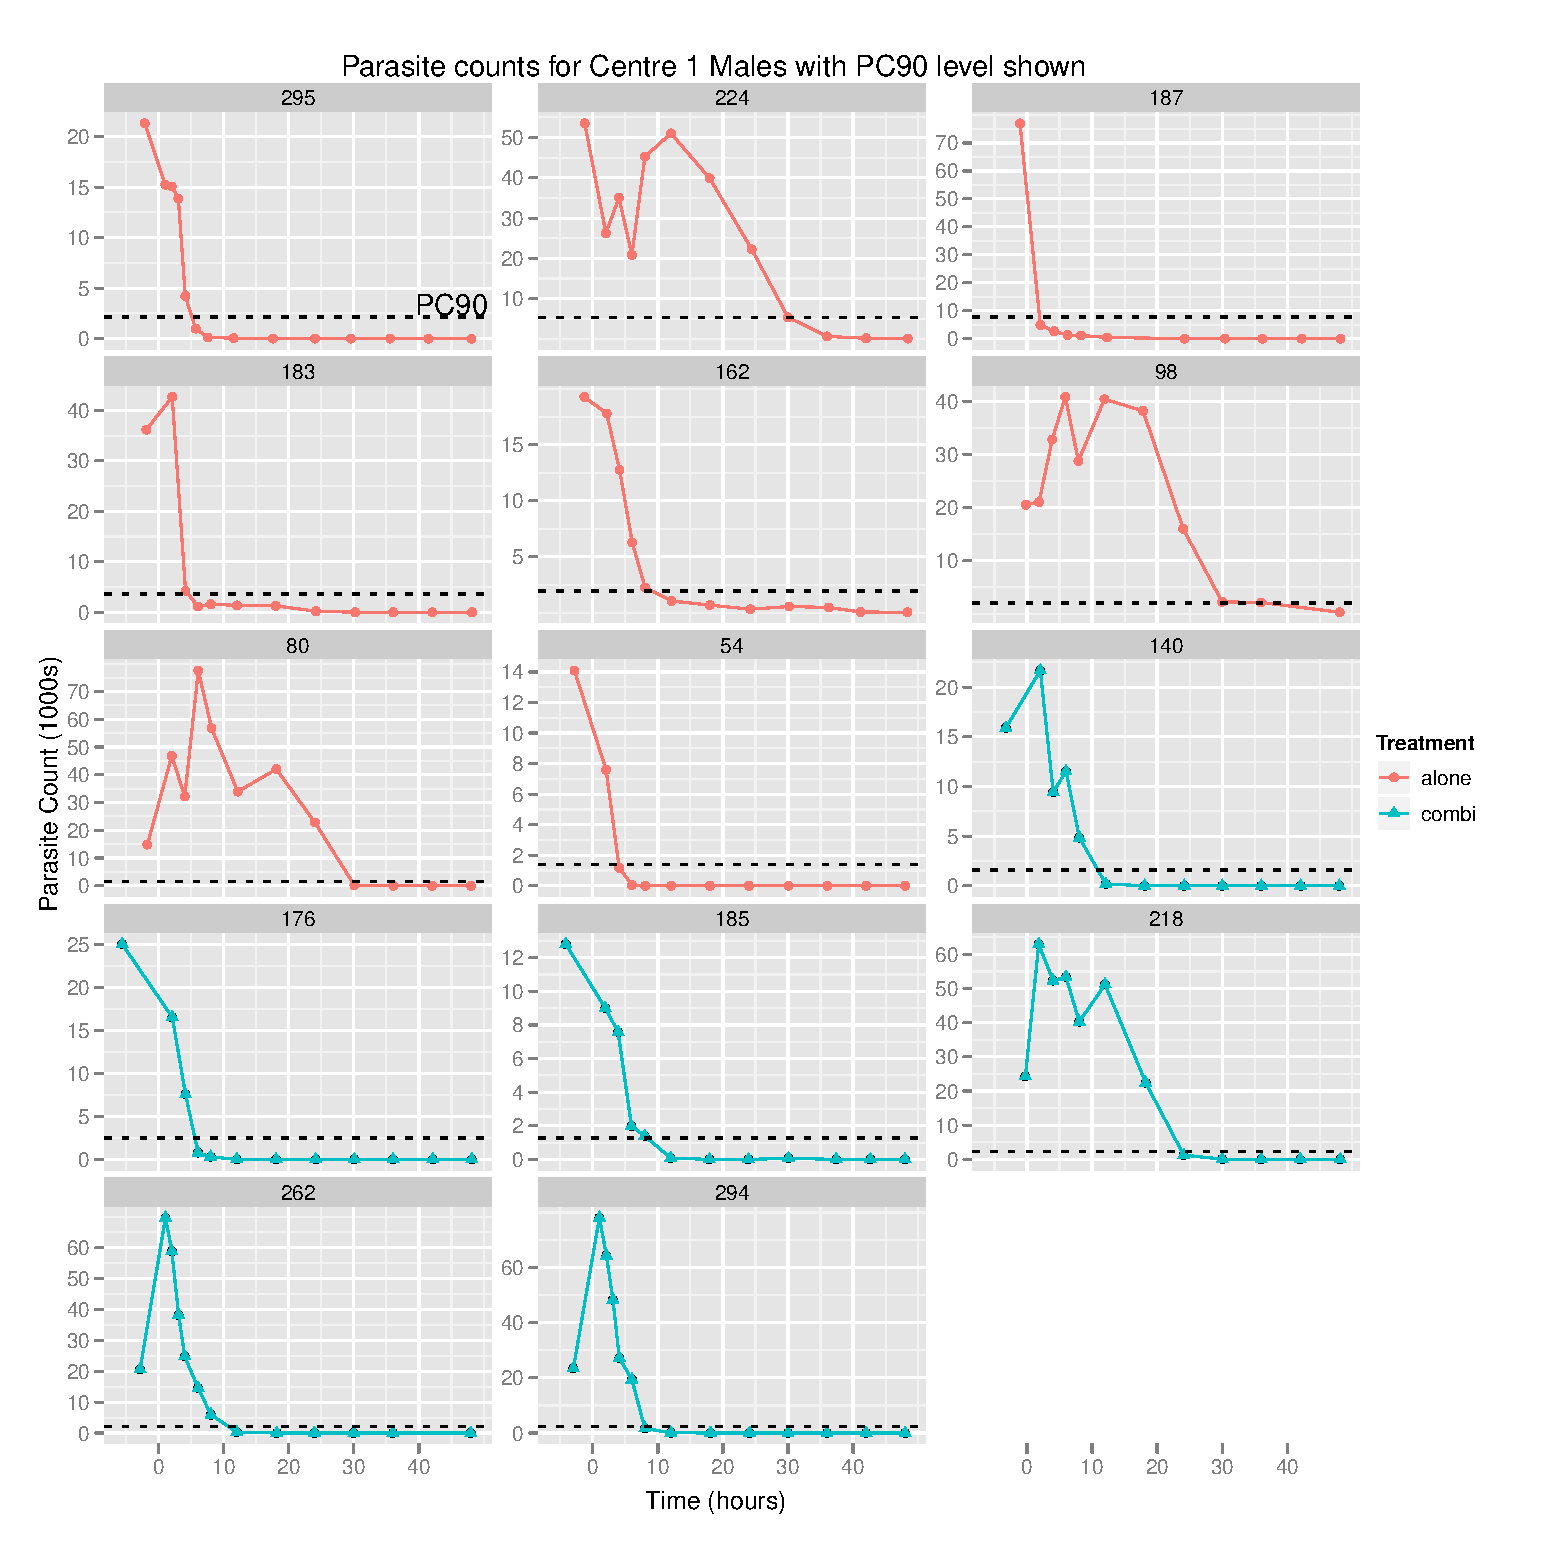
\includegraphics[width=6.1in]{raw901M.eps}
\caption{Untransformed parasite counts with PC90 level shown}
\label{raw901M}
\end{center}
\end{figure}
\begin{figure}[p]
\begin{center}
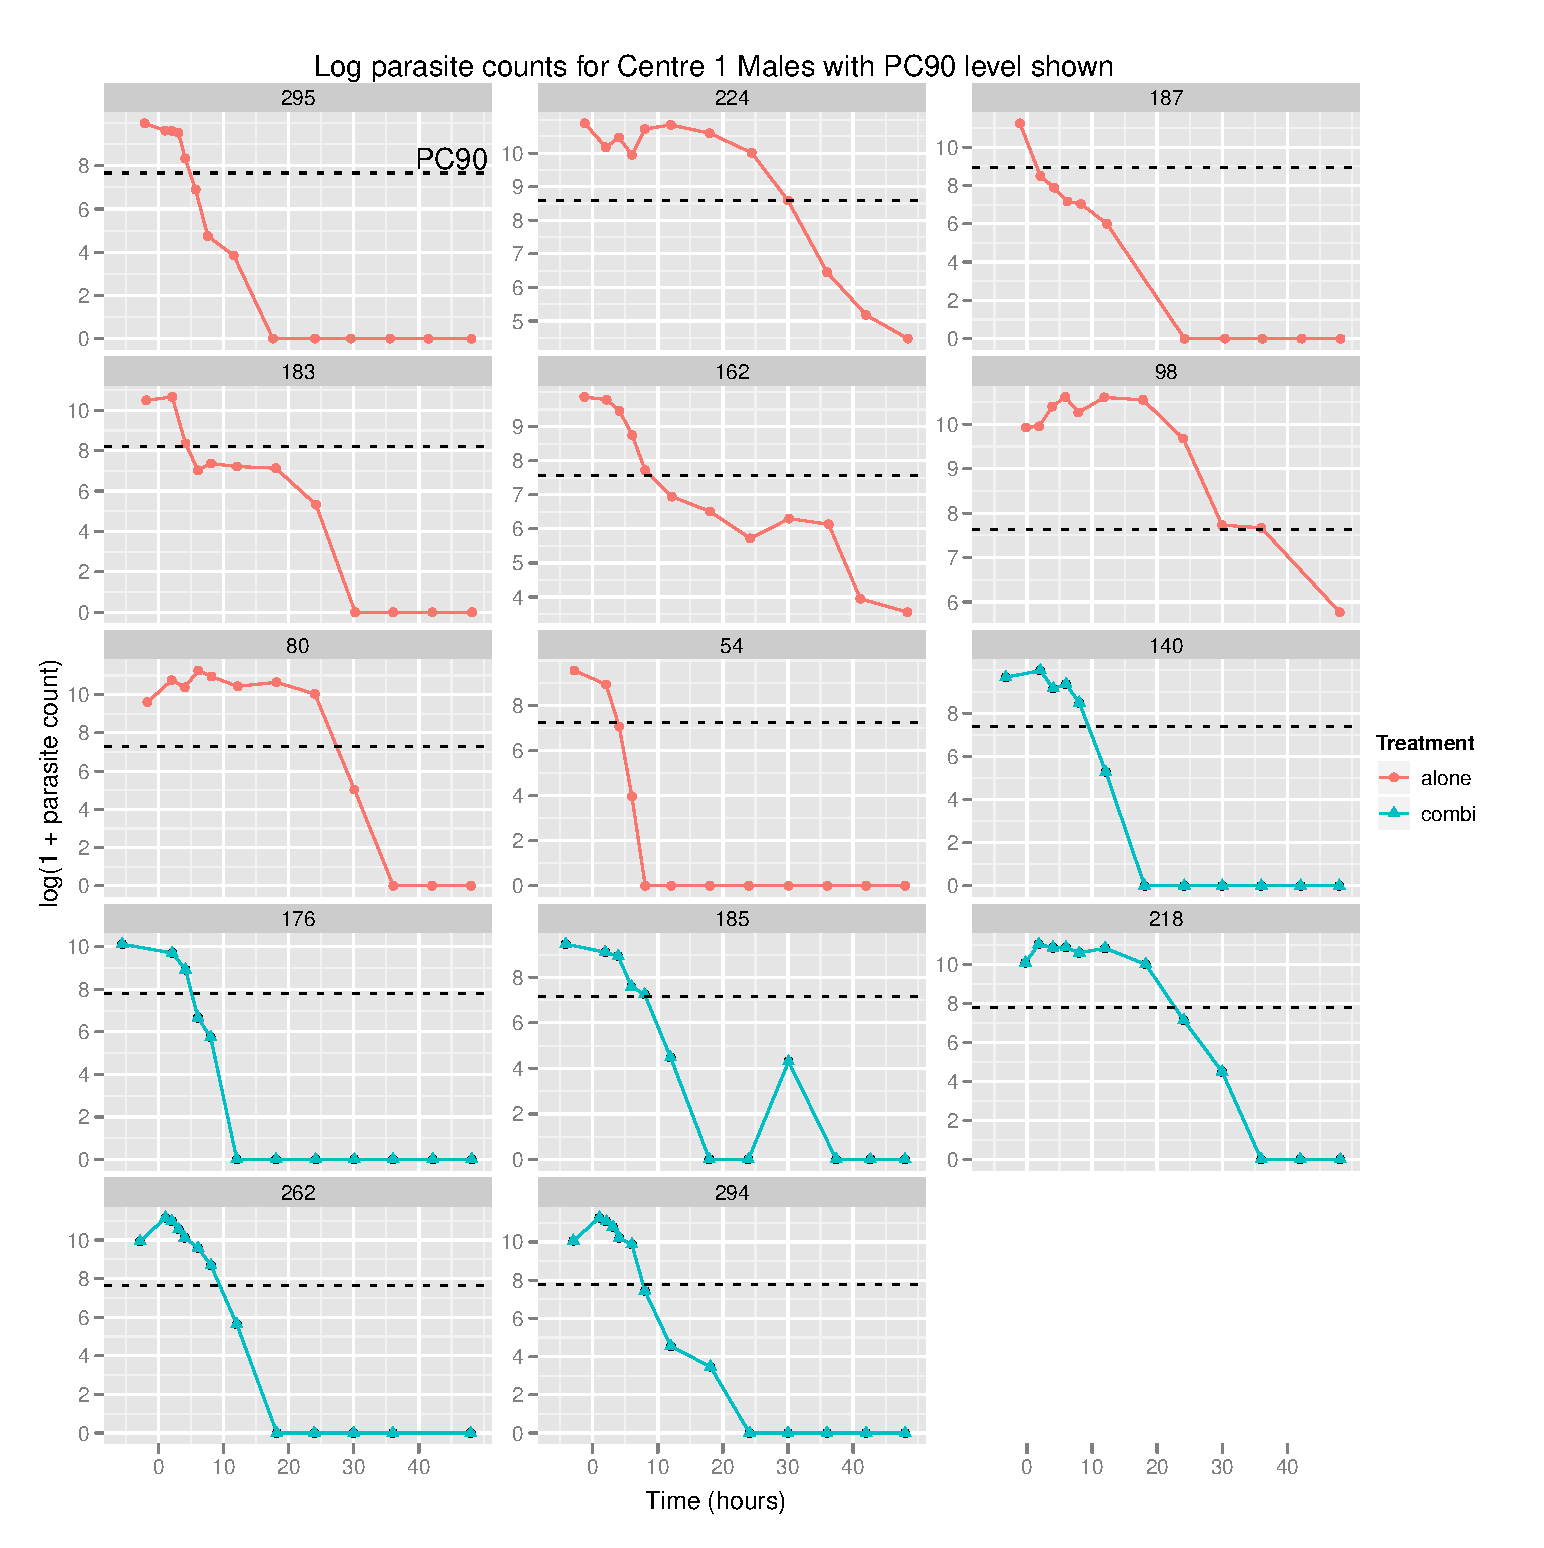
\includegraphics[width=6.1in]{log901M.eps}
\caption{Log parasite counts with PC90 level shown}
\label{log901M}
\end{center}
\end{figure}
\section{Estimation techniques}
\subsection{Polynomial linear regression}
It was found that a cubic polynomial was the most suitable model, if we include the data only up to the first zero parasite count. For some patients where the parasite count drops quickly to zero a fit that includes the subsequent run of zeroes would pull the cubic fit away from the most sensible estimate of PC90. It is more suitable for the purpose of estimating PC90 to only model the drop in the count to zero.

A cubic model was fitted to the log-transformed parasite count $P_{t}$ with time from first dose $t$ as the explanatory variable thus
$$\log(1+P_{t})=\beta_0+\beta_1t+\beta_2t^2+\beta_3t^3+\epsilon\quad\quad\epsilon\sim N(0,\sigma^2)$$
where $\log(1+P_{t})$ is used so that the dependent variable is zero at zero parasite count.

Figure \ref{cubics} shows the cubic fits to the log parasite count for centre 1, male subjects. It can be seen that the model describes the data fairly well, but it looks as if the combined treatment data is more closely modelled, with the single treatment data showing more dispersion about the fitted model. 
\begin{figure}[p]
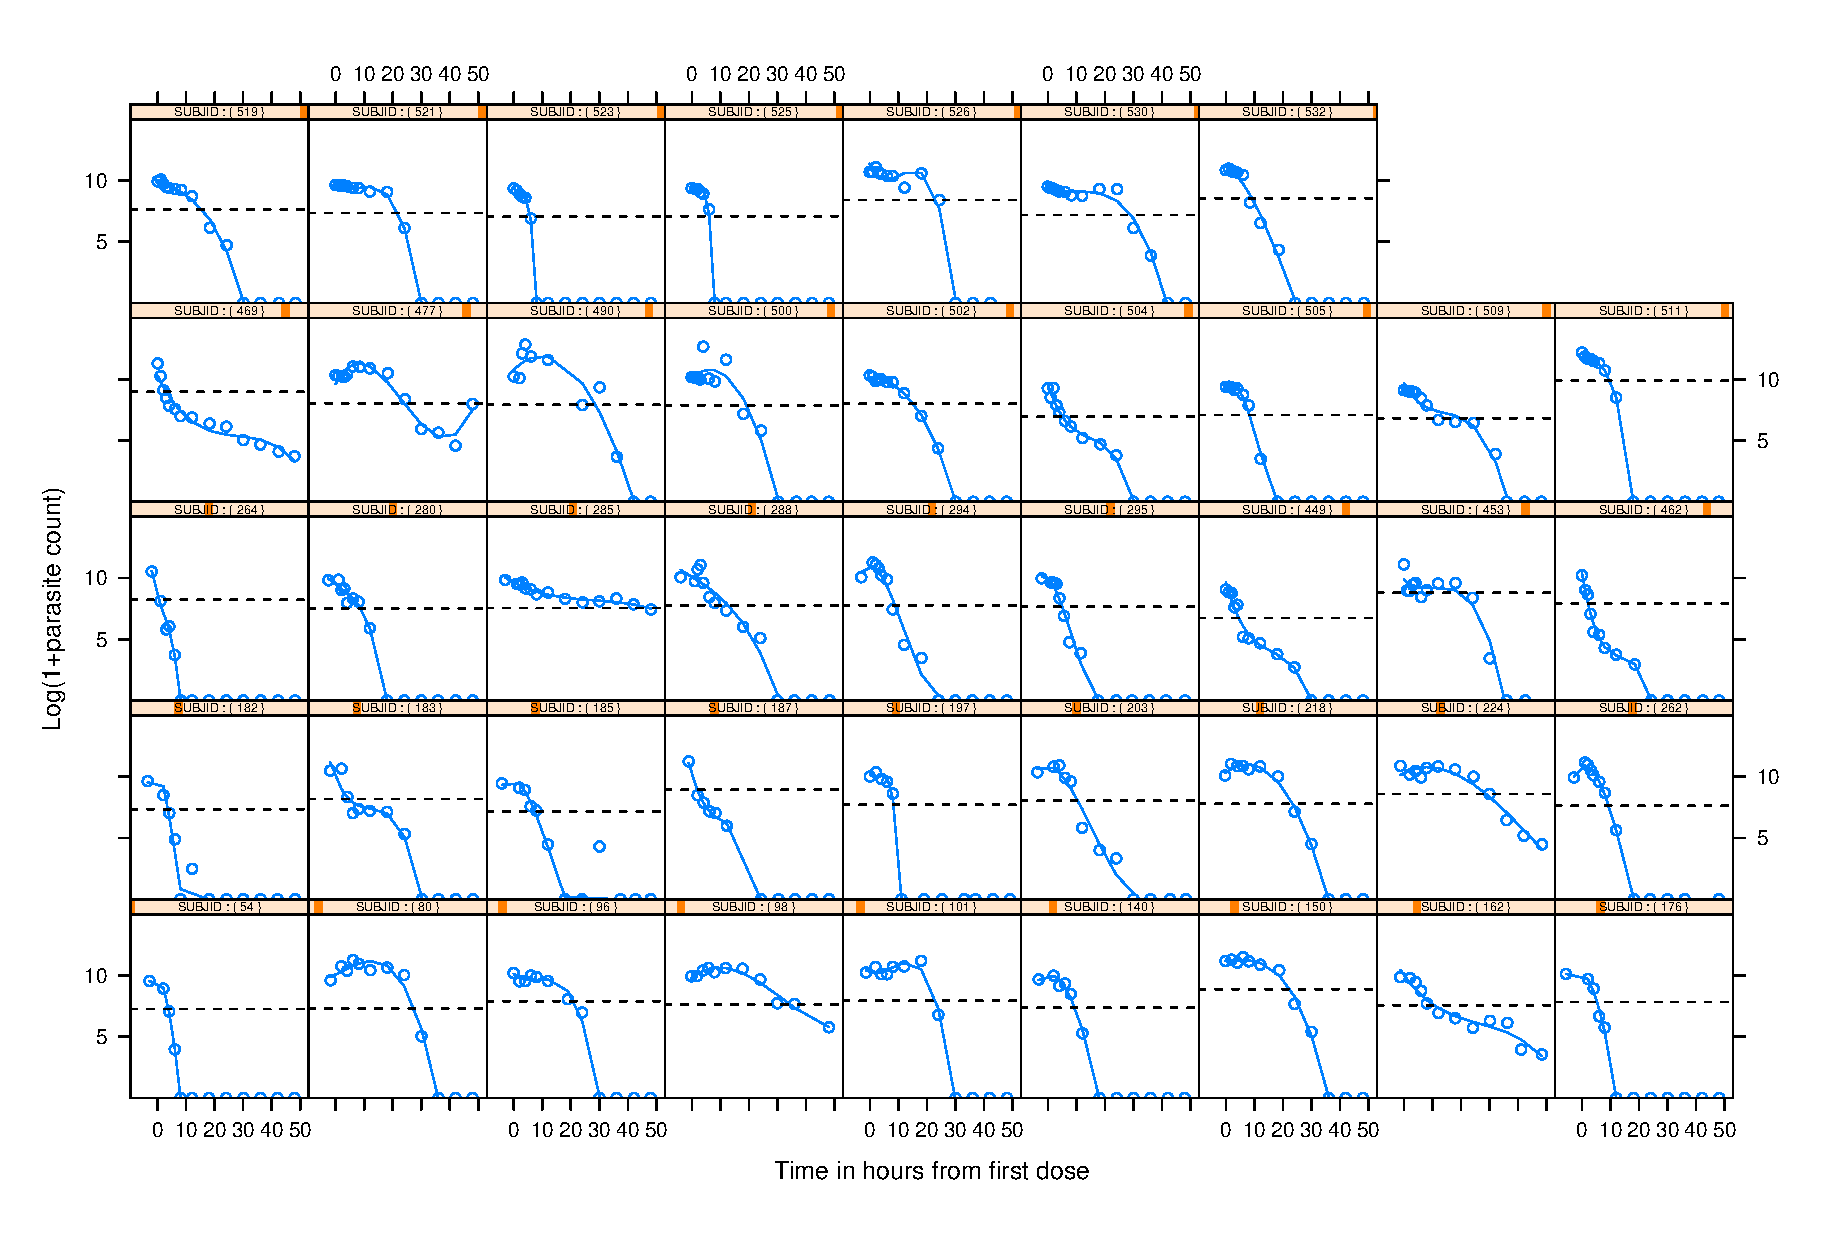
\includegraphics[width=6.1in]{cubics.eps} 
\caption{Cubic fits to log parasite count up to first zero reading}\label{cubics}
\end{figure}

Figure \ref{cubicsresid} shows the standardized residuals ($e/\hat{\sigma}$) for the cubic fits.
\begin{figure}[h]
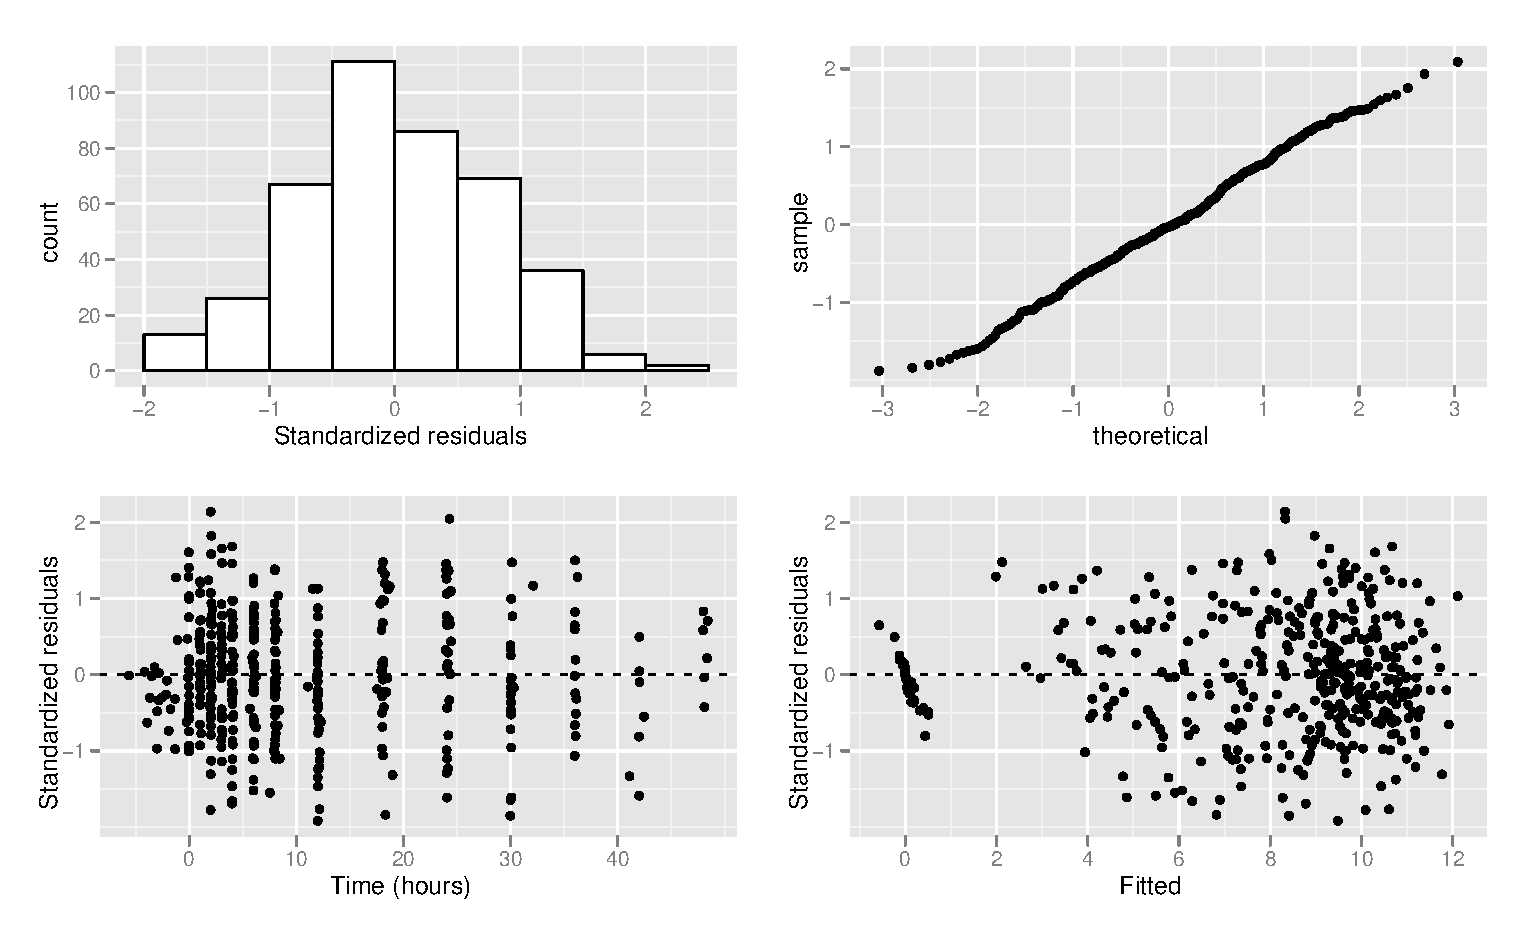
\includegraphics[width=6.1in]{cubicsresid.eps} 
\caption{Standardized residuals for cubic fits}\label{cubicsresid}
\end{figure}
It can be seen that they are normally distributed and show no obvious correlation with time from first dose or with fitted count. The cluster of small magnitude residuals at zero fitted value occurs because, in the fitting, this datum is not random but always zero each subject. Strictly this invalidates the assumptions of the fitted model but there isn't a more suitable choice for determining the shape. The cubic model is really only used as a convenient method of interpolation and we are not interested in inference regarding the fitted parameters as long as there is no systematic bias. 
\subsubsection*{Determining PC90 from the fitted model}
The value of PC90 i.e. the time t at which the parasite count has fallen to 10\% was found by finding the positive root of the cubic equation
$$\hat{\beta_0}-\hat{\beta_1}t-\hat{\beta_2}t^2-\hat{\beta}_3t^3-0.1{P_{0}}=0$$
that lies within our time period, where $P_0$ is the pre-treatment parasite count, $t$ is the time from first dose and $\hat{\beta_i}$ are the fitted coefficients for the cubic model. This root was found numerically using the \emph{R} \texttt{uniroot} function\cite{R}, which takes as an argument the interval over which to search for the root.
\pagebreak
\subsection{Non-linear logistic regression}
The logistic model as, used by Wootton \textit{et al}.\cite{wootton}, is
$$\log(1+P_t)=\alpha+\frac{\lambda}{1+e^{-\beta(t-\mu)}}+\epsilon\quad\quad\epsilon\sim N(0,\sigma^2)$$
This was fitted to all the data as it can model a drop from an initial count level to a level of zero, unlike the cubic model. $\alpha$ is the lower asymptote which we would expect to be zero. $\alpha+\lambda$ is the upper asymptote which we would generally expect to be $P_0$ except in the cases where there is a marked increase in the parasite count after the first dose. $\beta$ determines the rate of reduction with time and $\mu$ is the point of inflection (maximum rate of reduction). This model was fitted using the \emph{R} non-linear least-squares function \texttt{nls}\cite{R}. Logistic fits to the same subjects as the cubic fits in Figure \ref{cubics} are shown in Figure \ref{logistics}.
\begin{figure}[p]
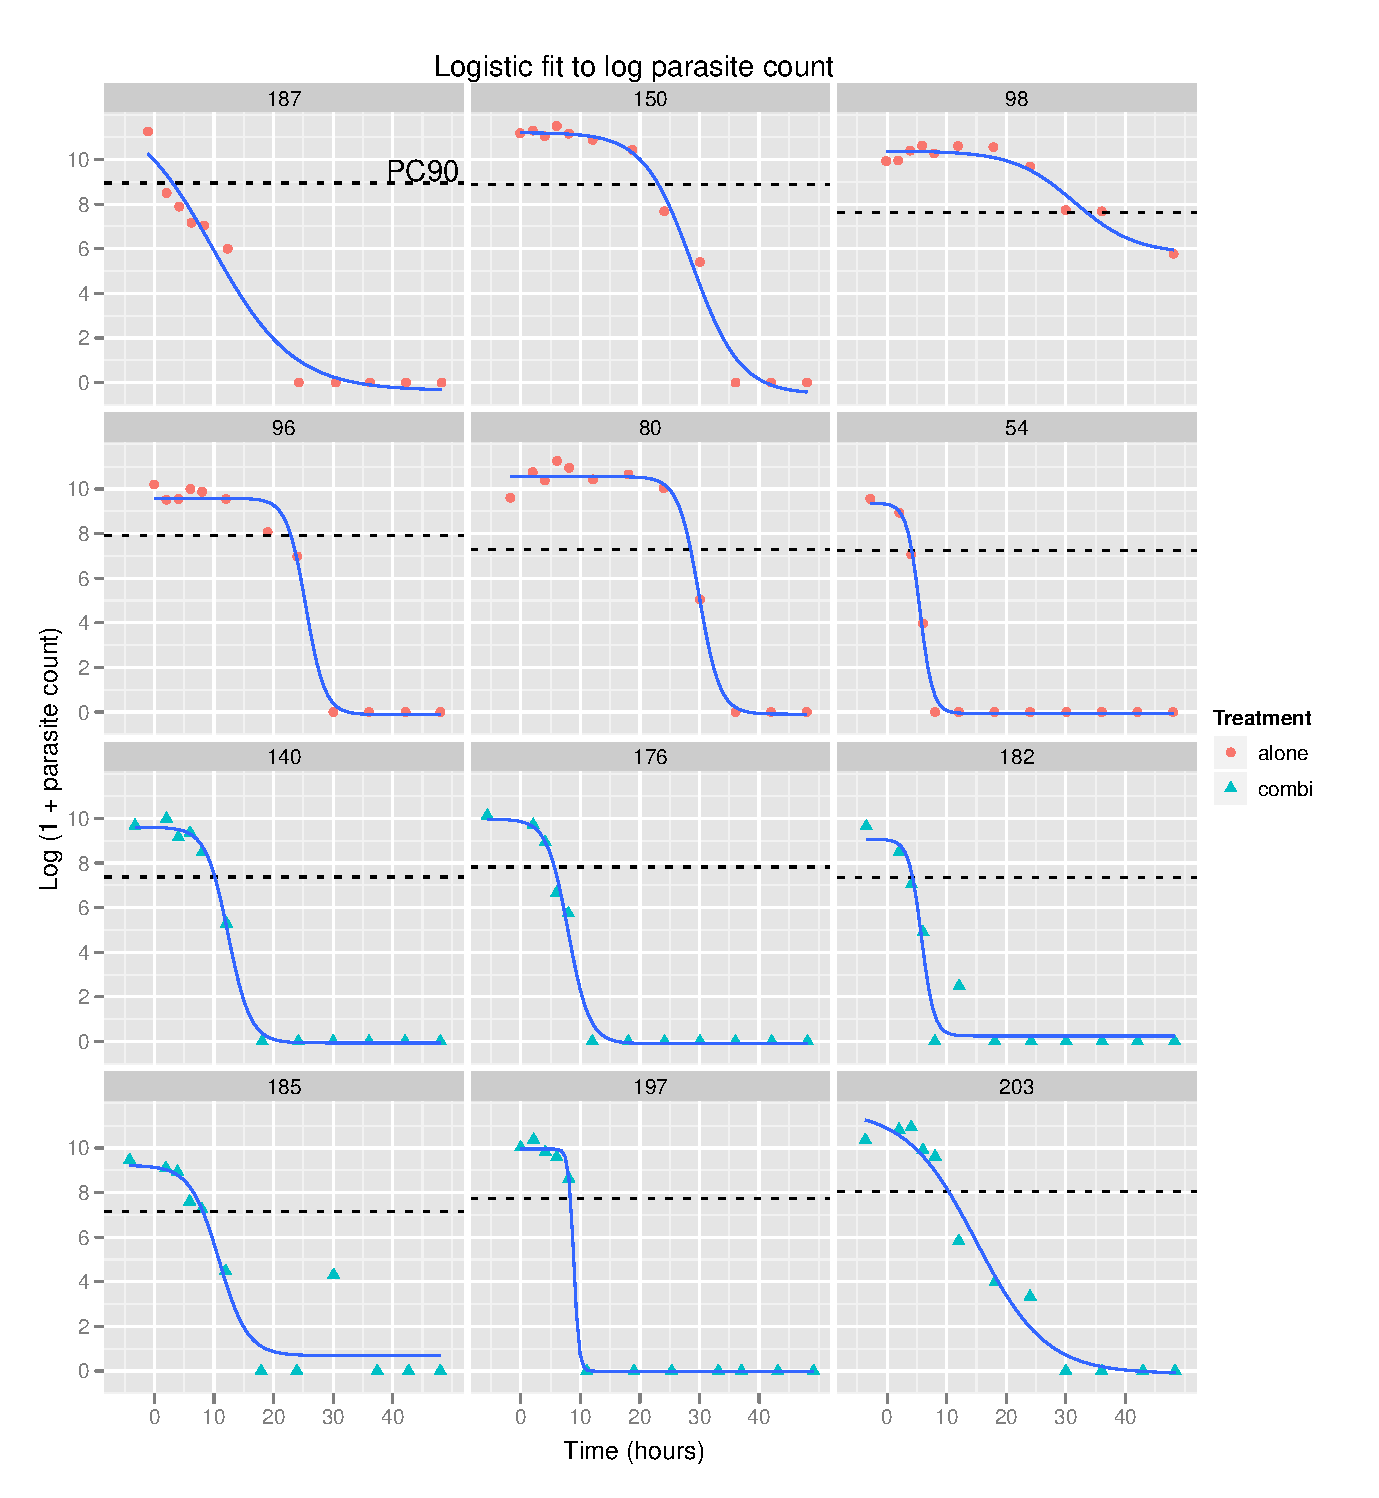
\includegraphics[width=6.5in]{logistics.eps} 
\caption{Logistic fits to log parasite count}\label{logistics}
\end{figure}

It can be seen that the logistic model describes the data about as well as the cubic model for these subjects except perhaps slightly worse for subject 96 and slightly better for subject 80.

If we look at the standardized residuals from the logistic fitting in Figure \ref{logisticresid} we can see that the logistic model is not an appropriate statistical model for this data. The residuals are not normally distributed and they are correlated with time and fitted parasite count. Again, inclusion of the run of non-random zero counts is partially responsible for this. However, this does not entirely invalidate this approach as all we are really concerned with here is a method that will automatically give us a sensible PC90 estimate in the region of interest; formulating an appropriate statistical model of the behaviour over the whole time period not the aim here.
\begin{figure}[h]
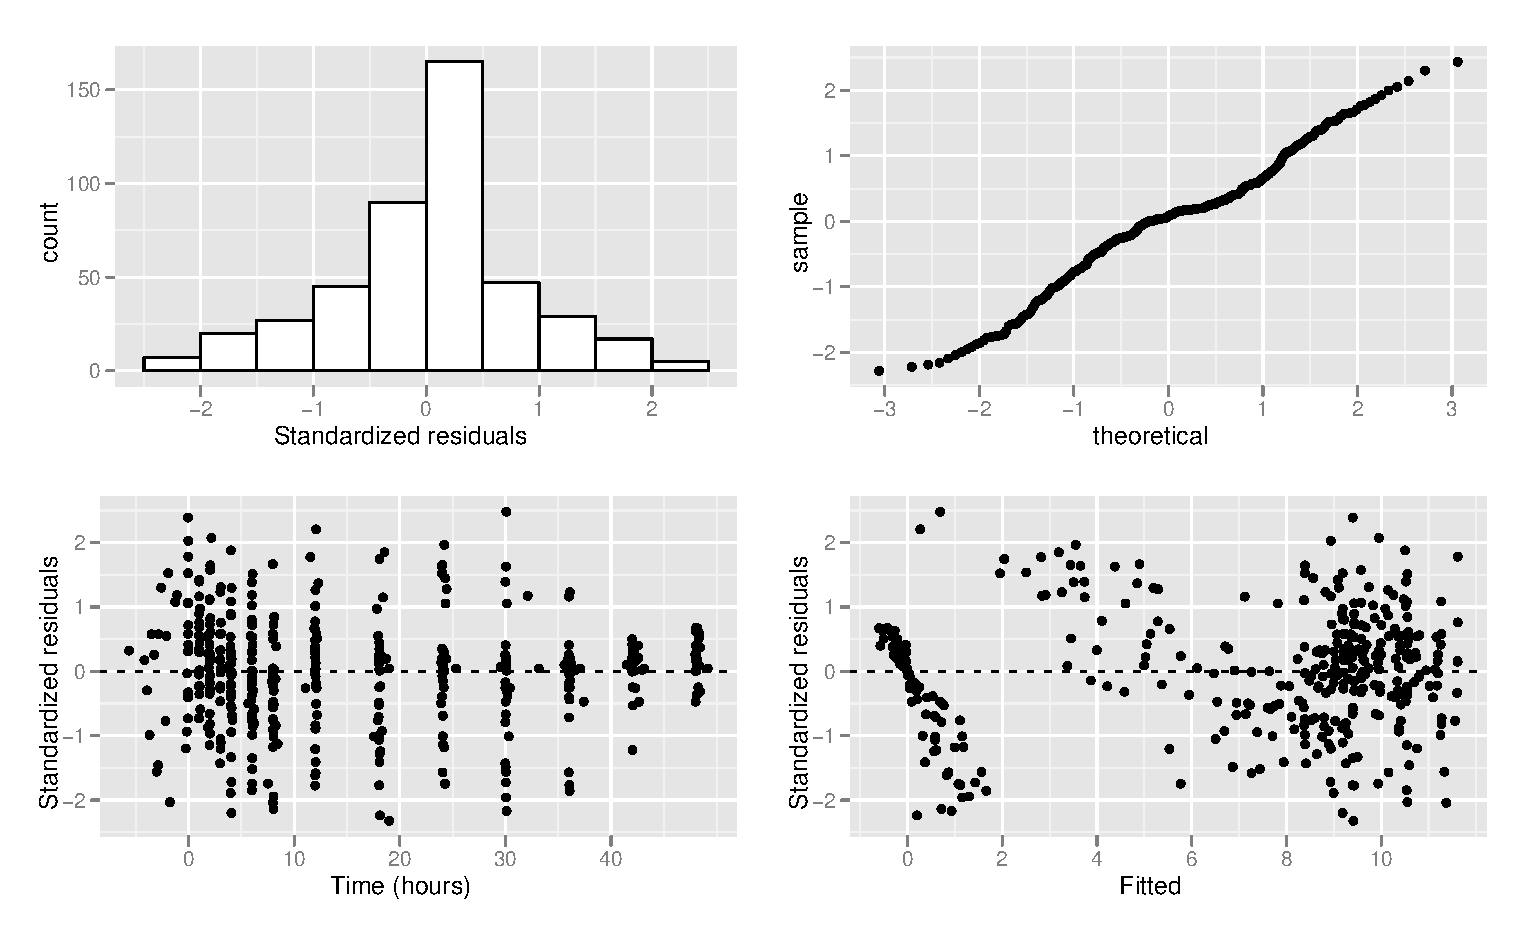
\includegraphics[width=6.5in]{logisticresid.eps} 
\caption{Standardized residuals for logistic fits}\label{logisticresid}
\end{figure}
\subsubsection*{Determining PC90 from the fitted model}
As before the \emph{R} \texttt{uniroot} function was used to find $t$ lying within our time period satisfying the equation
$$\log(1+P_t)=\hat{\alpha}+\frac{\hat{\lambda}}{1+\exp[-\hat{\beta}(t-\hat{\mu})]}-0.1{P_{0}}=0$$
where $\hat{\alpha}$, $\hat{\lambda}$, $\hat{\beta}$ and $\hat{\mu}$ are the fitted coefficients of the model.
\subsubsection*{Choosing starting values for the parameters}
Figure \ref{logparms} shows the roles the parameters of the logistic model play in shaping the fitted curve. The \texttt{nls} non-linear, least-squares fitting routine can take starting values for the parameters to be estimated.
\begin{figure}[h]
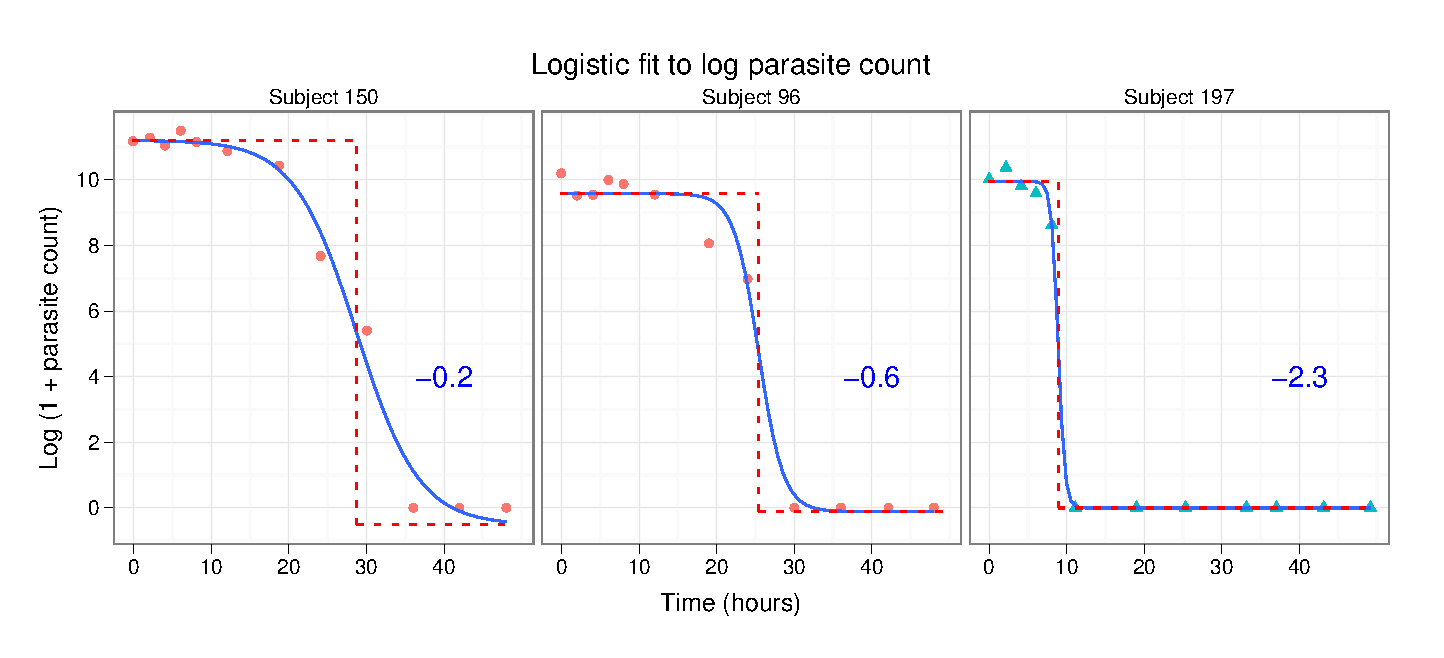
\includegraphics[width=6.1in]{logparms.eps} 
\caption{Illustration of parameters for logistic fits.\newline
The horizontal red lines show $\log(1+P_t)=\alpha$ (lower) and $\log(1+P_t)=\alpha+\lambda$ (upper), the vertical red line shows $t=\mu$ and the coefficient $\beta$ (rate of reduction) is given in blue.}\label{logparms}
\end{figure}
Looking at Figure \ref{logparms} it clearly follows that sensible starting values are:
\begin{itemize}
\item $\alpha$ = the minimum parasite count; usually 0.
\item $\lambda$ = the maximum minus the minimum count; usually the maximum.
\item $\mu$ = the time corresponding to the parasite count closest to halfway between the maximum and minimum counts.
\end{itemize} 
It was found by experimentation that the most suitable starting value for $\beta$ was -0.5, but that the fitting was insensitive to choice of $\beta$ if varied over the range of fitted $\beta$ values observed (and somewhat beyond).
\subsubsection*{Failure of logistic fitting}
Despite careful selection of starting parameters, it was found for several subjects that a logistic model is simply not appropriate. In these cases either the non-linear fitting routine failed to converge or, if convergence criteria were relaxed, would fit a model highly dependent on choice of starting parameters which, when plotted with the data, obviously does not model the data satisfactorily. The data for these subjects where logistic fitting failed are shown in Figure \ref{failures}.
\begin{figure}[h]
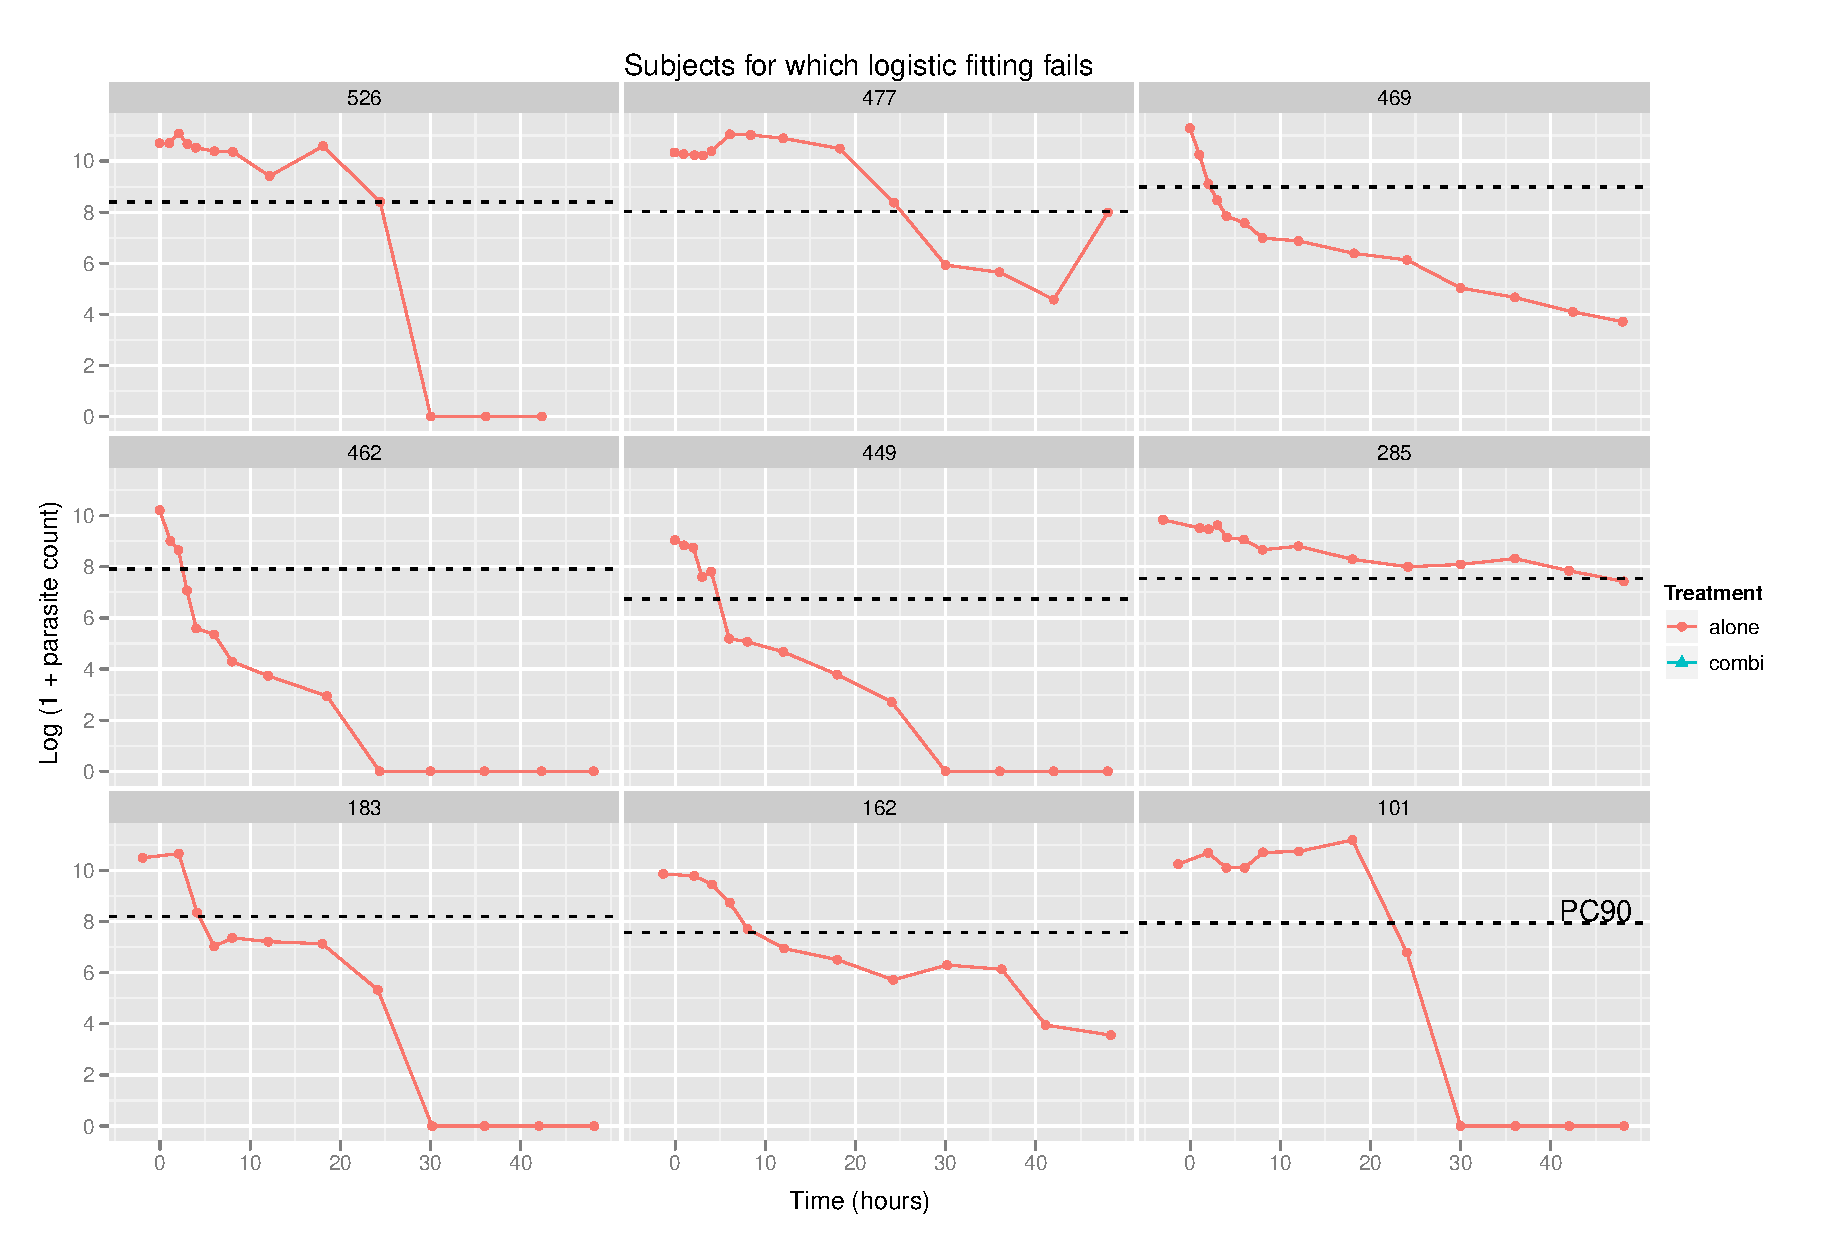
\includegraphics[width=6.1in]{failures.eps} 
\caption{Subjects for which the logistic fitting fails}\label{failures}
\end{figure}

It is interesting to note that all subjects for which logistic fitting fails are in the single treatment group; $p=0.0039$ under the null hypothesis of equal probability of a subject being from the single or combined treatment group using a binomial model. This is evidence that the parasite counts for patients on the single treatment follow more varied trajectories during clearance compared to patients on the combined treatment whose clearance can consistently be described with a logistic or cubic model to a reasonable approximation.

In addition to parasite count profiles that simply do not conform to a logistic shape there were subjects where insufficient data in the region between the upper and lower asymptotes meant that logistic fitting was inappropriate. For example, subjects 526 and 101 in Figure \ref{failures}, where choice of different starting parameters for $\mu$ and $\beta$ would result in different logistic fits being obtained. One possible fit having a steep transition (large absolute $\beta$), whereby the data at the upper and lower levels is closely modelled. Another possible fit having a shallower transition (smaller $\beta$) that models the slope of a line passing through the ends of the run of points at the upper and lower levels and the point in the middle, but  has a less severe curvature such that the corners at the upper and lower levels are poorly modelled. In summary the fit is free to rotate about the single point between the upper and lower levels and thus cannot be suitably defined.
\subsection{Log-linear interpolation}
The datum immediately above the PC90 level is joined with a straight line to the datum immediately below the PC90 level in on a plot of $\log(1+P_{t})$ against time. The point where this line crosses the PC90 level determines $t$=PC90.
\section{Comparison of estimation methods}
Table \ref{PC90} shows a comparison of the PC90 estimates obtained by the 3 different methods utilised so far.
\begin{table}[p]
\centering
\caption{Comparison of PC90 estimated by 3 methods}\label{PC90}
\begin{tabular}{|cccc|rrr|}
\hline
Subject&Centre&&&PC90&PC90&PC90\\
ID&ID&Sex&Treatment&cubic&logistic&log-linear\\
\hline
54&Centre 1&Male&alone&3.82&4.14&3.85\\
80&Centre 1&Male&alone&27.62&28.50&27.32\\
96&Centre 1&Female&alone&21.18&22.95&19.76\\
98&Centre 1&Male&alone&34.50&33.51&36.30\\
101&Centre 1&Female&alone&23.20&-&22.45\\
140&Centre 1&Male&combi&9.47&10.16&9.47\\
150&Centre 1&Female&alone&22.52&23.12&21.75\\
162&Centre 1&Male&alone&10.54&-&8.84\\
176&Centre 1&Male&combi&5.32&5.66&5.05\\
182&Centre 1&Female&combi&3.98&4.29&3.65\\
183&Centre 1&Male&alone&4.55&17.21&4.35\\
185&Centre 1&Male&combi&7.59&8.13&8.10\\
187&Centre 1&Male&alone&1.81&3.05&1.53\\
197&Centre 1&Female&combi&8.38&8.35&8.40\\
203&Centre 1&Female&combi&10.48&10.30&9.69\\
218&Centre 1&Male&combi&23.48&23.92&22.77\\
224&Centre 1&Male&alone&28.86&30.26&30.01\\
262&Centre 1&Male&combi&9.40&9.85&9.40\\
264&Centre 1&Female&combi&0.37&1.43&0.85\\
280&Centre 1&Female&combi&8.76&9.72&9.04\\
285&Centre 1&Female&alone&47.74&-&46.52\\
288&Centre 1&Female&combi&12.86&12.38&9.38\\
294&Centre 1&Male&combi&8.86&8.68&7.73\\
295&Centre 1&Male&alone&5.02&4.98&4.83\\
449&Centre 2&Male&alone&4.45&-&4.82\\
453&Centre 2&Female&alone&19.66&23.08&21.97\\
462&Centre 2&Female&alone&2.11&-&2.49\\
469&Centre 2&Male&alone&3.01&-&2.21\\
477&Centre 2&Female&alone&24.03&-&25.08\\
490&Centre 2&Female&alone&28.73&29.94&31.63\\
500&Centre 2&Male&combi&19.36&19.66&17.15\\
502&Centre 2&Female&combi&15.33&16.33&14.77\\
504&Centre 2&Female&alone&5.07&6.64&5.00\\
505&Centre 2&Female&combi&8.26&9.02&8.75\\
509&Centre 2&Male&alone&20.59&18.63&11.59\\
511&Centre 2&Male&combi&10.00&10.91&9.51\\
519&Centre 2&Male&combi&15.63&16.08&14.68\\
521&Centre 2&Female&alone&22.14&23.38&21.64\\
523&Centre 2&Female&combi&5.82&5.97&5.84\\
525&Centre 2&Female&combi&6.15&6.17&6.23\\
526&Centre 2&Female&alone&23.48&-&24.42\\
530&Centre 2&Male&alone&29.10&29.28&28.09\\
532&Centre 2&Male&combi&9.16&9.21&8.08\\
\hline
\end{tabular}
\end{table}
\pagebreak
\subsection{Graphical comparison}
Figure \ref{pc90-agree} shows 8 examples of subjects where estimation by the 3 different methods shows good agreement. It seems likely that the differences between these estimates are of a comparable scale to experimental error. It can be seen that the 3 methods give close agreement when the data can be closely modelled by cubic or logistic fitting and when the gradient of the log-linear interpolation is similar to the regression models in the region around PC90. 
\begin{figure}[h]
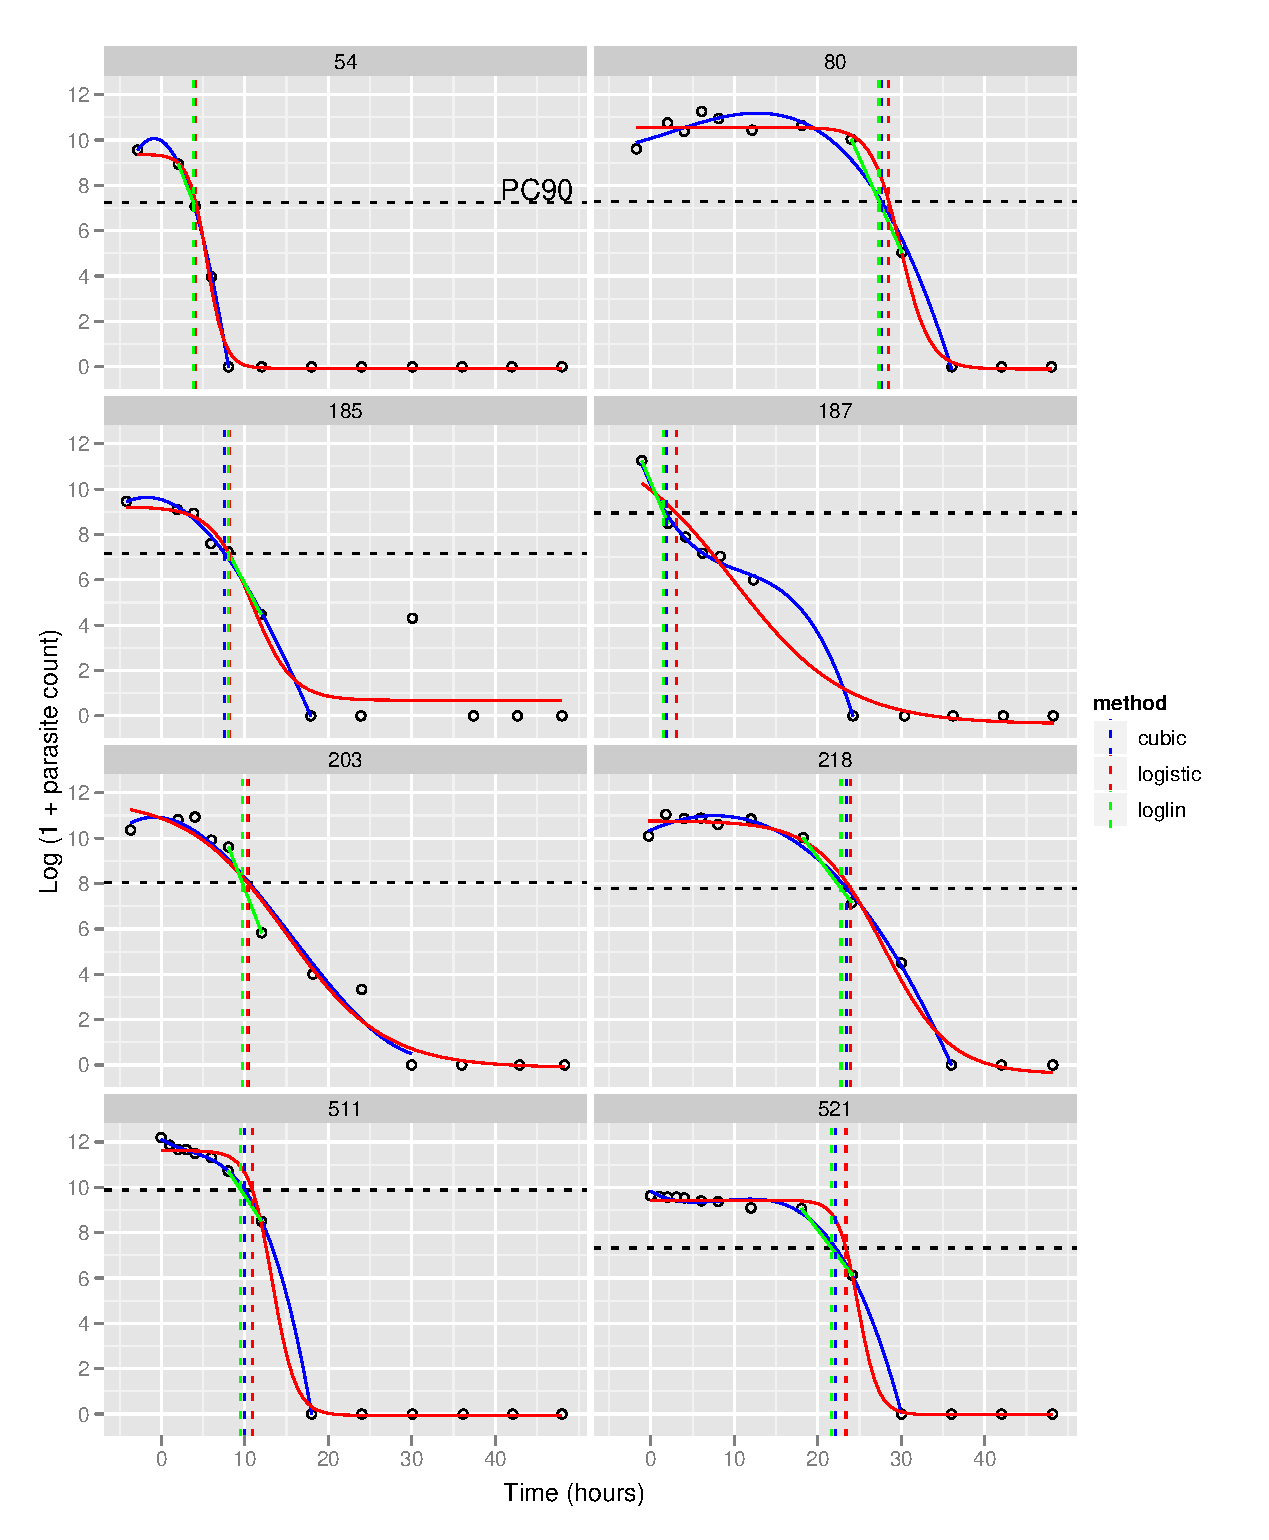
\includegraphics[width=6.5in]{pc90-agree.eps} 
\caption{Subjects with little difference in PC90 estimated by 3 methods}
\label{pc90-agree}
\end{figure}

Figure \ref{pc90-bad} shows examples of subjects where estimation by the 3 different methods has resulted in notable differences between PC90 estimates. These differences appear to arise when:
\begin{enumerate}
\item The drop in parasite count is slow or stationary around the PC90 level e.g. subjects 98, 183, 453 and 509. In these cases the regression lines and interpolation may cross the PC90 level at markedly different times. In subject 183 this has given a difference in PC90 between the logistic and other two methods of over 10 hours.
\item There is ``unusual'' data near the PC90 level e.g. subjects 490 and 500 where recorded counts, seemingly off the prevailing trend, have influenced the interpolated estimate.
\end{enumerate}
\begin{figure}[h]
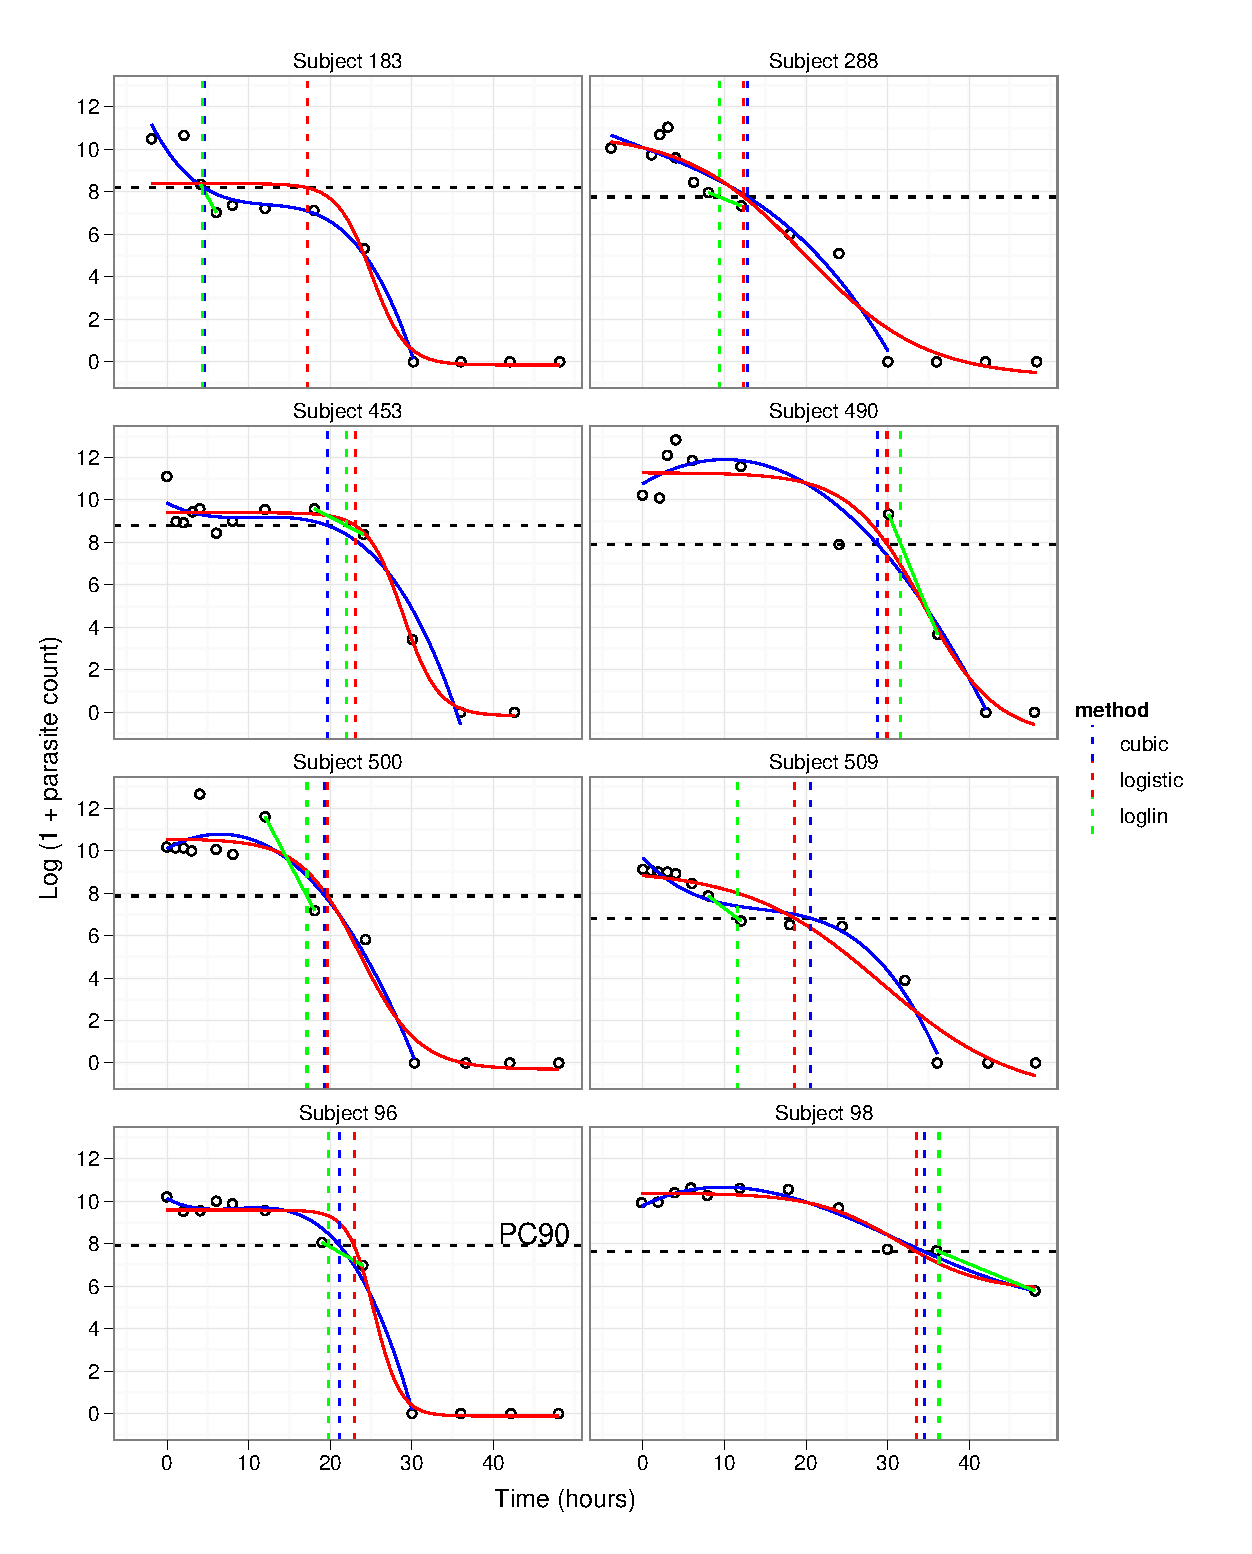
\includegraphics[width=6.5in]{pc90-bad.eps} 
\caption{Subjects with notable difference in PC90 estimated by 3 methods}
\label{pc90-bad}
\end{figure}
Figure \ref{pc90-nofit} shows the cubic and log-linear interpolated estimates for subjects where logistic fitting was inappropriate.
\begin{figure}[h]
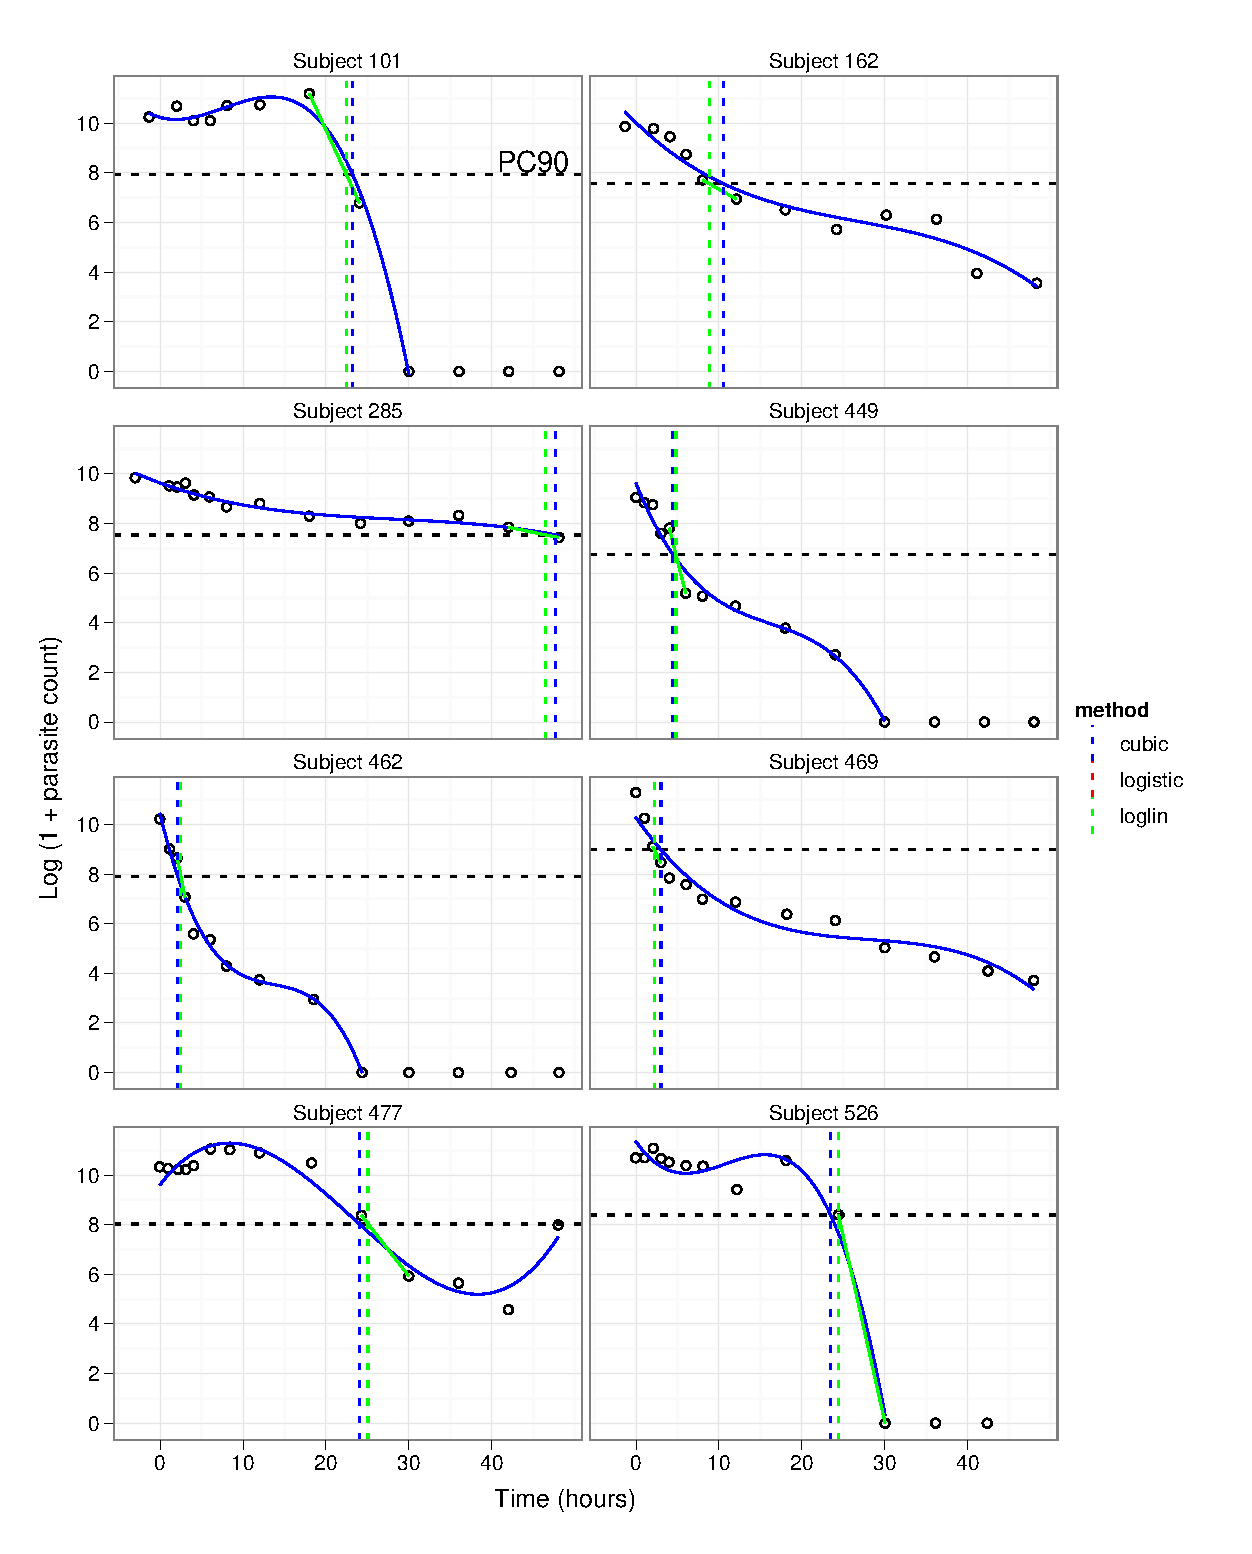
\includegraphics[width=6.5in]{pc90-nofit.eps} 
\caption{PC90 estimation for subjects where logistic fitting was inappropriate}
\label{pc90-nofit}
\end{figure}
It can be seen that the two methods in these cases appear to produce very similar estimates.
\clearpage
\subsubsection*{Between and within subjects comparisons}
Figure \ref{methodsbysubject} shows the distribution of PC90 estimates for each method in two ways:
\begin{enumerate}
\item ``Between subjects'' simply shows the distributions of PC90 estimates.
\item ``Within subjects'' removes the effect of correlation between estimates made on the same subject by showing the distribution of the difference of the PC90 estimate from the subject mean.
\end{enumerate}
\begin{figure}[p]
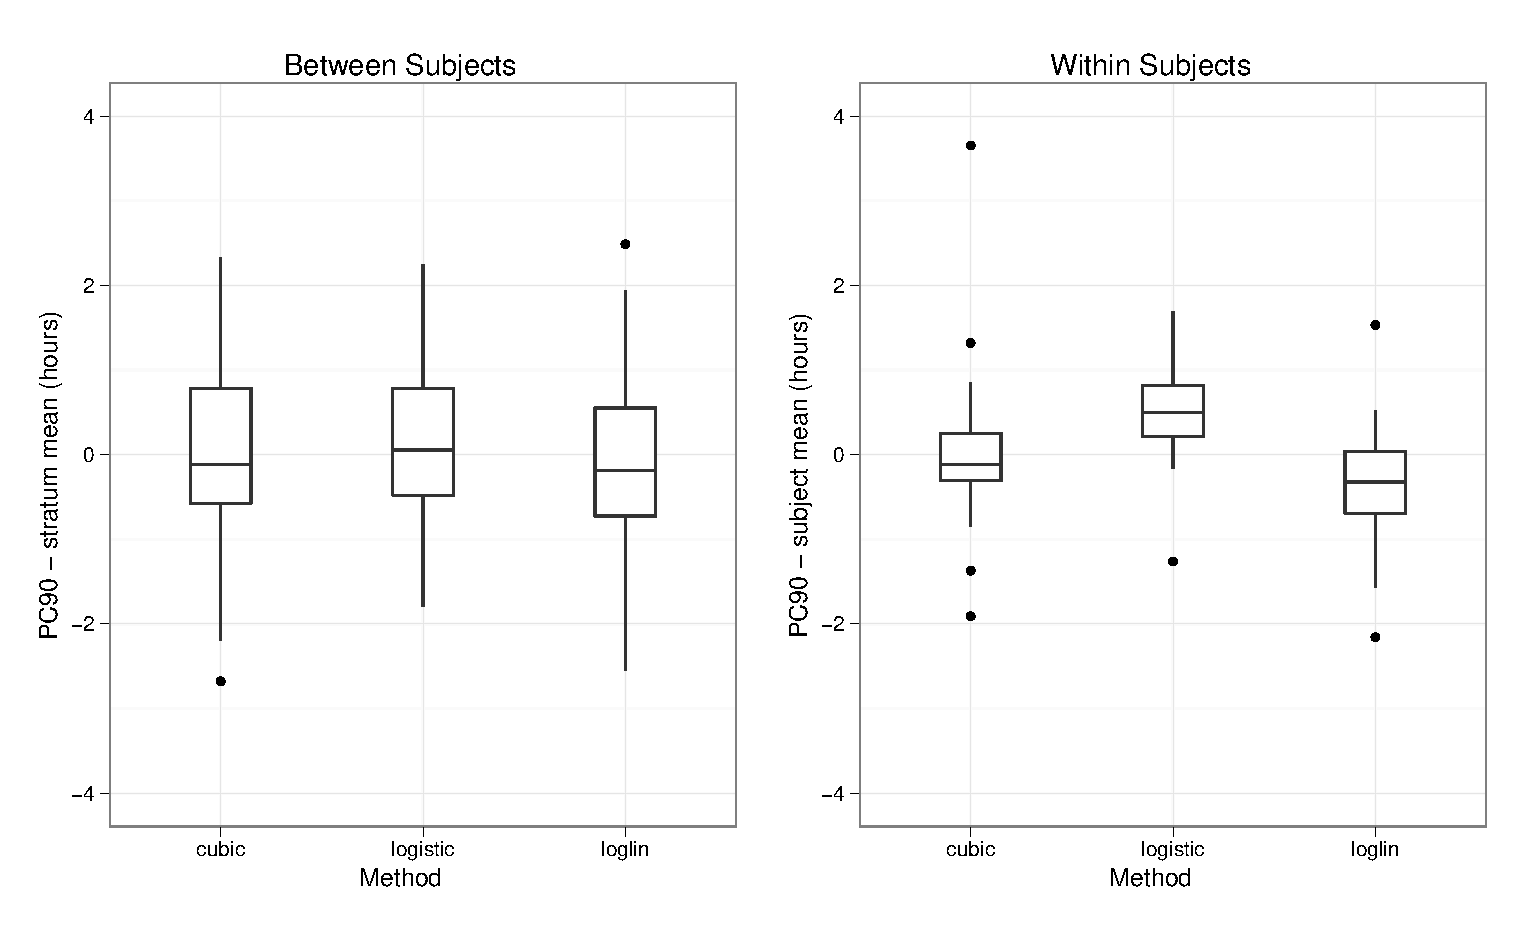
\includegraphics[width=6.5in]{methodsbysubject.eps} 
\caption{Comparison of PC90 estimates between and within subjects}
\label{methodsbysubject}
\end{figure}
It can be seen that the choice of method only seems to have a significant effect within subjects with the logistic method appearing to give estimates higher than average and the log-linear interpolation method slightly lower. This suggests that variance between methods is only significant within subjects.
% \subsubsection{Interaction of estimation method with experimental factors}
% Figures \ref{methodsbycentre}, \ref{methodsbysex} and \ref{methodsbytreatment} show the between and within subject PC90 estimates split by experimental factors centre, sex and treatment respectively:
% \begin{itemize}
% \item There does not seem to be any significant difference in the relationship between the 3 methods between centres.
% \item Sex does not appear to alter the relationship between the 3 methods.
% \item The three methods perhaps show closer agreement on the combined treatment.
% \end{itemize}
% In summary it does not seem that there are any significant interactions between the experimental factors and the estimates produced by the 3 methods.
% \begin{figure}[p]
% \includegraphics[width=6.5in]{methodsbycentre.eps} 
% \caption{Comparison of PC90 estimates by centre}
% \label{methodsbycentre}
% \end{figure}
% \begin{figure}[p]
% \includegraphics[width=6.5in]{methodsbysex.eps} 
% \caption{Comparison of PC90 estimates by sex}
% \label{methodsbysex}
% \end{figure}
% \begin{figure}[p]
% \includegraphics[width=6.5in]{methodsbytreatment.eps} 
% \caption{Comparison of PC90 estimates by treatment}
% \label{methodsbytreatment}
% \end{figure}
\pagebreak
\subsection{Statistical comparison}
%If we perform 2-way ANOVA between the 3 PC90 estimates by subject and method i.e.
%$$\mathrm{PC}90_{ij}=subject_{i}+method_{j}+\epsilon_{ij}\quad\quad\epsilon\sim N(0,\sigma^{2})$$ 
%we obtain the residuals shown in Figure \ref{pc90resid}.
%It can be seen that there are several outlying data points at up to $4\sigma$ and almost $8\sigma$. These correspond to subjects 183 and 509 for whom we obtained very different PC90 estimates by the 3 methods. As can be seen in Figure \ref{pc90-bad}, this is due to the parasite count being fairly constant around the PC90 level for these subjects.
%
%If we repeat the ANOVA analysis with subjects 183 and 509 removed, we obtain the residuals shown in Figure \ref{pc90resid-sub}.
%It can be seen that the residuals are approximately normally distributed with no obvious structure except for perhaps a smaller variance at smaller PC90 times. The results of the ANOVA analysis are shown in Table \ref{pc90aov}.
%\begin{table}[h]
%\centering
%\caption{ANOVA comparison of PC90 estimated by 3 methods}\label{pc90aov}
%\begin{tabular}{l|rrrrr}
%Source&Sum Sq.&df&Mean Sq.&$F$&P($>F$)\\
%\hline
%Subject&12023.7&40&300.6&558.8&$<1\times 10^{-15}$\\
%Method&12.1&2&6.0&11.2&$5.7\times 10^{-5}$\\
%Residual&38.7&72&0.54&&\\
%\hline
%Total&12074.5&114&&&
%\end{tabular}
%\end{table}
To perform a statistical comparison between the PC90 estimation methods we want to test the null hypothesis that the difference between PC90 estimated by each method is zero. In order to do this we need to look at the distribution of the differences between PC90 estimates and accordingly choose an appropriate statistical test.
\subsubsection*{Distributions of differences}
\begin{description}
\item[Cubic and logistic methods] - The distribution of the difference between PC90 estimated by the cubic and logistic methods is shown in Figure \ref{cub-log}. Apart from one outlying datum it can be seen that the differences are approximately normally distributed. The outlying value corresponds to subject 183, which we can see in Figure \ref{pc90-bad} gives a very different estimate by the two methods due to the parasite count being fairly constant around the PC90 level.
\item[Cubic and log-linear interpolation methods] - The distribution of the difference between PC90 estimated by the cubic and log-linear interpolation methods is shown in Figure \ref{cub-loglin}.
Again the distribution is approximately normally distributed apart from a single outlying value corresponding to subject 509. We can see in Figure \ref{pc90-bad} that again this corresponds to estimates made in a region where the parasite count is flat.
\item[Logistic and log-linear interpolation methods] - The distribution of the difference between PC90 estimated by the logistic and log-linear interpolation methods is shown in Figure \ref{log-loglin}. The two outlying values correspond to subjects 183 and 509 again.
\end{description}
As the distributions of differences are all approximately normally distributed, apart from a few anomalous estimates as described, we can used paired-sample $t$ tests to test our null hypothesis.
\begin{figure}[h]
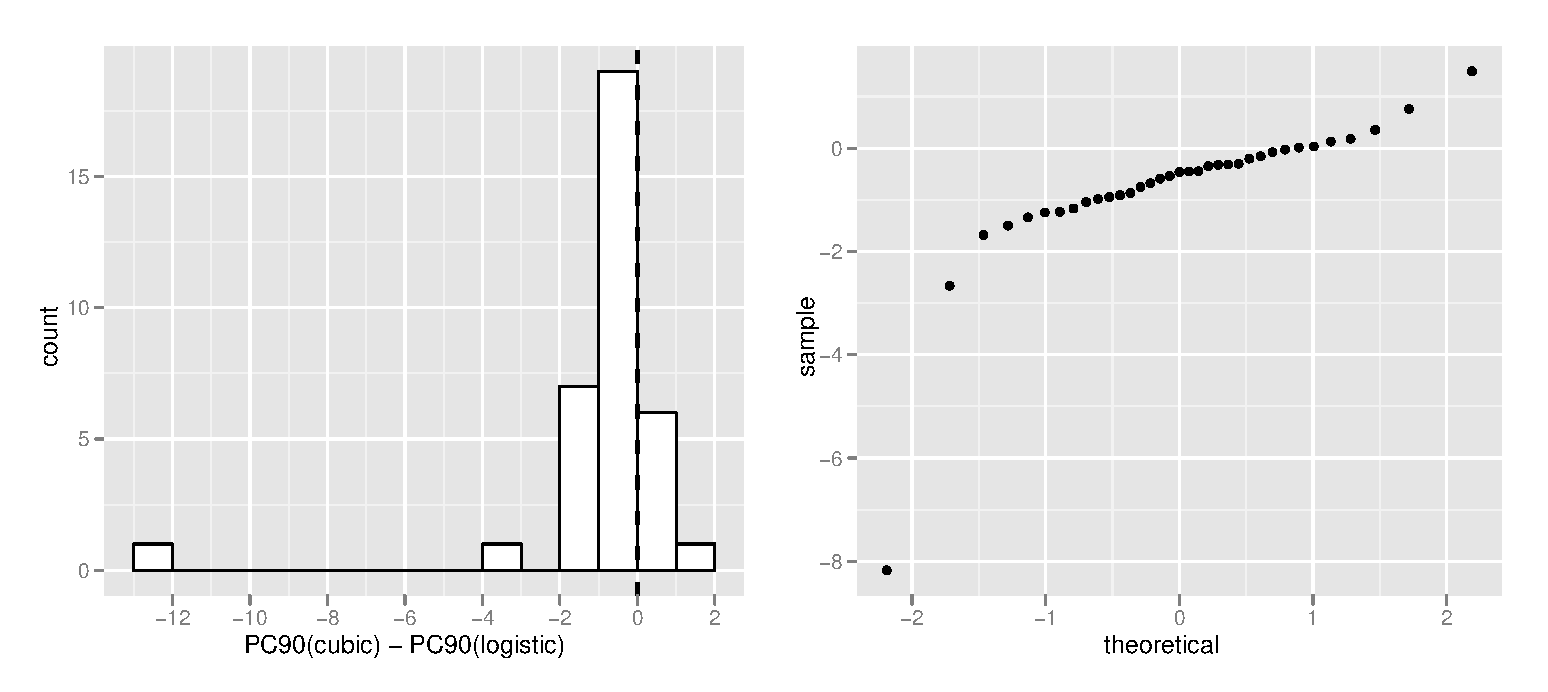
\includegraphics[width=6.5in]{cub-log.eps} 
\caption{Distribution of the difference between PC90 estimated by the cubic and logistic methods}
\label{cub-log}
\end{figure}
\begin{figure}[p]
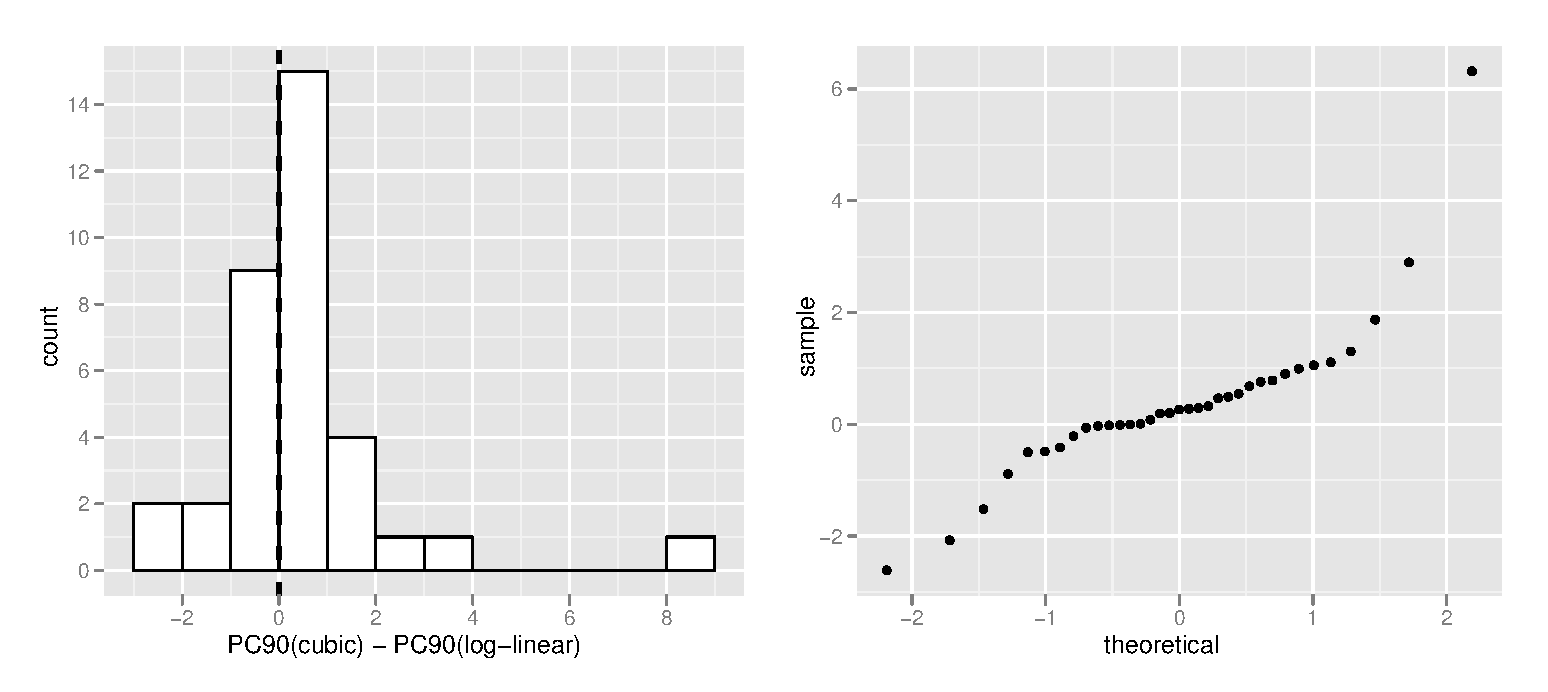
\includegraphics[width=6.5in]{cub-loglin.eps} 
\caption{Distribution of the difference between PC90 estimated by the cubic and log-linear interpolation methods}
\label{cub-loglin}
\end{figure}
\begin{figure}[p]
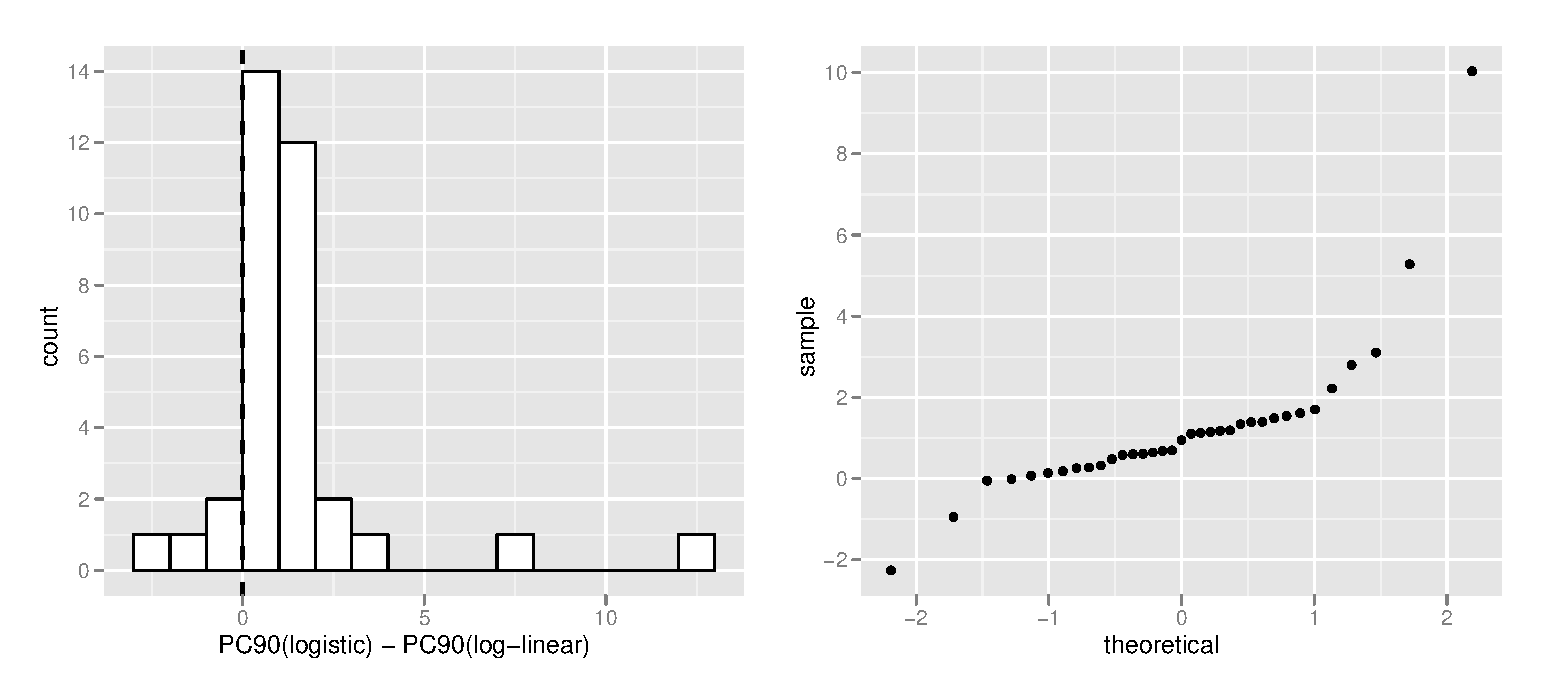
\includegraphics[width=6.5in]{log-loglin.eps} 
\caption{Distribution of the difference between PC90 estimated by the logistic and log-linear interpolation methods}
\label{log-loglin}
\end{figure}
\subsubsection*{Paired $t$ tests}
\begin{description}
\item[Cubic and logistic methods] - If we perform a paired $t$ test between PC90 estimated by the cubic and logistic methods, excluding subject 183, we find good evidence to reject the hypothesis that the two methods result in the same PC90 estimate ($P<0.005$). On average the logistic method gives PC90 32 minutes longer than the cubic method with a 95\% confidence interval of (13, 51) minutes, bearing in mind this is only based on a comparison of the subset of 35 subjects for which a logistic fit was possible out of the total of 43.
\item[Cubic and log-linear interpolation methods] - A paired $t$ test excluding subject 509 gives no evidence to reject the hypothesis that the cubic and log-linear interpolation methods give the same PC90 estimates.
\item[Logistic and log-linear interpolation methods] - A paired $t$ test excluding subjects 183 and 509 gives good evidence to reject the hypothesis that the logistic and log-linear methods produce the same PC90 estimates ($P<0.0005$). On average the logistic method produces PC90 estimates 49 minutes longer than the log-linear interpolation method with a 95\% confidence interval of (25, 73) minutes.
\end{description}
\subsubsection*{ANOVA}
The results of 4-way ANOVA on the 121 PC90 estimates (3 estimates for each of 43 subjects, minus 8 where no logistic estimate could be made), classified by estimation method, centre, sex and treatment with all interactions are shown in Table \ref{pc90aov}. Only the results for the effect of the PC90 method used and its 2-way interactions are shown here so as not to pre-empt the analysis of the next chapter; 3-way and higher interactions were all non-significant.
\begin{table}[h]
\centering
\caption{ANOVA comparison of PC90 estimated by 3 methods}\label{pc90aov}
\begin{tabular}{l|rrrrr}
Source&Sum Sq.&df&Mean Sq.&$F$&P($>F$)\\
\hline
$Method$&7.2&2&3.6&0.041&$0.96$\\
$Method\times Centre$&61.0&2&30.5&0.35&$0.71$\\
$Method\times Sex$&119.2&2&59.6&0.68&0.51\\
$Method\times Treatment$&10.0&2&5.0&0.057&0.94\\
$\vdots$&$\vdots$&$\vdots$&$\vdots$&$\vdots$&$\vdots$\\
$Residuals$&8517.1&97&87.8&&\\
\hline
Total&12340.86&120&&&
\end{tabular}
\end{table}

It can be seen that there is no evidence that the variance in PC90 between estimation methods is any larger than the variance between subjects in each centre-sex-treatment stratum. Therefore the difference between PC90 estimates is independent of other factors. The full results of the relative effects of all factors can be found in the next chapter. At this stage we are just concerned with the effect of choice of PC90 estimation method.

In summary the $t$ tests show us that the difference between methods is significant within subjects for 2 out of the 3 comparisons. The ANOVA analysis shows that it is insignificant in comparison to the variation due to centre, sex and treatment.
\subsubsection*{Correlation of difference with magnitude}
We have deduced from the 4-way ANOVA with interactions that there is no interaction between the method chosen and the other factors that influences the PC90 estimation. The $t$ tests told us the average amount that the methods differ, if at all, and in which direction, but we should check if the difference between the methods is related to the size of the PC90 estimates. The difference in PC90 estimate between the methods is plotted against the mean estimate in Figure \ref{pc90est-cor}.
\begin{figure}[h]
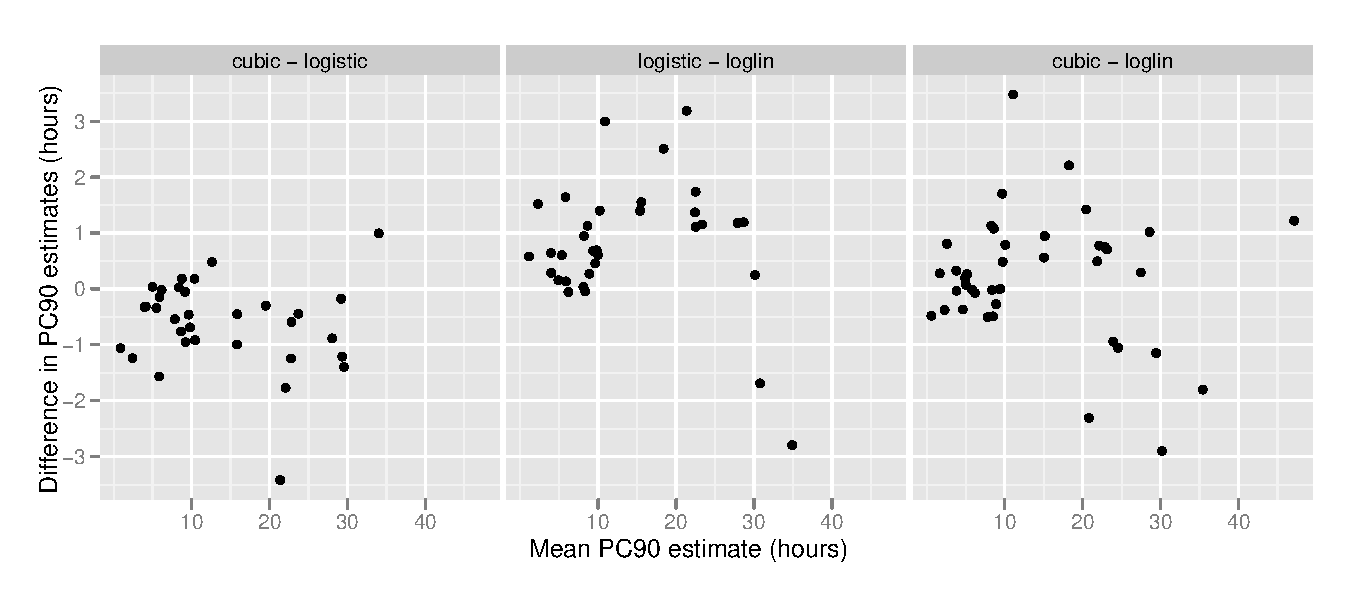
\includegraphics[width=6.5in]{pc90est-cor.eps} 
\caption{Difference in PC90 estimates against mean PC90 estimate}
\label{pc90est-cor}
\end{figure}

There is no obvious correlation and Spearman rank tests do not give any evidence to reject the null hypothesis of 0 correlation. This means that we can expect the methods to give PC90 estimates that differ by the amounts given by the $t$ tests independent of the size of the PC90 estimate.
\section{Key Results}
The key results from this investigation into methods for derivation of parasite clearance times are:
\begin{itemize}
\item The log-transformed parasite count from pre-dose up to the first zero count can be modelled by cubic polynomial linear regression. The combined treatment data seems to be more closely modelled by the cubic fit than the single treatment data.
\item The log-transformed parasite count can be modelled by a logistic non-linear model for 35 out of the 43 subjects. For the other 8 subjects it was found that a logistic model is inappropriate and ambiguous at best.
\item The subjects that could not be modelled by the logistic method were all from the single treatment group ($P<0.005$), indicating that patients on the single treatment show a different response to patients on the combined treatment.
\item A log-linear interpolation gives a simple alternative to regression methods for estimating PC90.
\item The cubic linear model and log-linear interpolation methods give statistically the same PC90 estimate averaged over all subjects: no evidence to reject null hypothesis of zero mean difference between PC90 estimates.
\item The logistic non-linear model produces PC90 estimates 32 minutes longer than the cubic method 
with a 95\% confidence interval of (13, 51) minutes.
\item The logistic method produces PC90 estimates 49 minutes longer than the log-linear interpolation method with a 95\% confidence interval of (25, 73) minutes.
\item The variance in PC90 between methods is insignificant compared to the variance in PC90 due to sex, centre and treatment.
\item The difference in PC90 due to estimation method is independent of sex, centre and treatment and magnitude of PC90. 
\end{itemize}
\subsection{Choice of PC90 estimation method}
The key advantages and disadvantages of each method are shown in Table \ref{pc90compare}.
\begin{table}[h]
\centering
\caption{Comparison of PC90 estimation methods}\label{pc90compare}
\begin{tabular}{|m{1.5in}|m{2.2in}|m{2.2in}|}
\hline
Method&Advantages&Disadvantages\\\hline
Cubic polynomial\newline linear regression&
\begin{list}{\labelitemi}{\leftmargin=1em}
\item Simple to fit.
\item Fits all subjects.
\item Fairly robust to erratic variation in PC90 region.
\end{list}&
\begin{list}{\labelitemi}{\leftmargin=1em}
\item Only models data up to first zero count.
\end{list}
\\\hline
Logistic non-linear\newline regression&
\begin{list}{\labelitemi}{\leftmargin=1em}

\item Models data over whole time period.
\item Fairly robust to erratic variation in PC90 region.
\end{list}&
\begin{list}{\labelitemi}{\leftmargin=1em}
\item Fitting procedure is complicated requiring choice of initial parameters.
\item Does not find a suitable fit for all subjects.
\end{list}
\\\hline
Log-linear\newline interpolation&
\begin{list}{\labelitemi}{\leftmargin=1em}
\item Simple to fit.
\item Fits all subjects.
\end{list}&
\begin{list}{\labelitemi}{\leftmargin=1em}
\item Only models PC90 region.
\item Sensitive to variation in PC90 region.
\end{list}
\\\hline
\end{tabular}
\end{table}

It appears that, for the purpose of PC90 estimation, there is little to choose between the cubic and log-linear interpolation methods. The cubic method will be more robust to the occurrence of spurious data in the PC90 region, although for the subjects studied here this does not seem to have greatly influenced estimates using log-linear interpolation. In fact if we look at subjects 500 and 509 in Figure \ref{pc90-bad} we see that although the log-linear interpolation differs from the other two estimates it has actually detected the time at which the primary endpoint is reached most accurately i.e. has produced an estimate closest to the first actual datum below the PC90 level.

There does not appear to be a compelling reason to use the logistic method. Although it perhaps models the behaviour at the upper and lower asymptotes better than the cubic method, it is not these regions that are of interest for estimating PC90. The fact that it is difficult to fit the logistic model and that it cannot fit almost 20\% of subjects also adds weight to using other methods.

The logistic model investigated here is the same one used by Wootton \textit{et al}.\cite{wootton}. However, they specify that the best model fit was chosen by two independent statisticians based on criteria such as the effect of outliers on the model fit and fit of the model in the baseline region. This is in contrast to the objective fit obtained here by use of computational fitting routines, the only input being starting parameters to help the routine arrive at a solution. Wootton \textit{et al}. discarded the data when no suitable logistic fit could be found. If these subjects were more likely to be from one treatment group, as we found here, this would unbalance the experiment.

Carmello \textit{et al}.\cite{carmello} use the log-linear interpolation method for estimating PC90. No studies using polynomial linear regression have been found.

In summary it would seem that the log-linear interpolation method seems the most suitable for estimating PC90, in terms of its simplicity and that it appears to consistently estimate sensible PC90 values as determined by graphical inspection. Perhaps estimates using the cubic method could also be easily computed and where the two methods disagree by a large amount e.g. greater than $3\sigma$ as for subject 509 here (Figures \ref{pc90-bad} and \ref{cub-loglin}), then these subjects could be flagged for closer inspection.

%\subsection{Other possible methods}
%One method of PC90 estimation that could combine the advantages of cubic and log-linear interpolation is 